% (Beamer Template) Copyright 2004 by Till Tantau <tantau@users.sourceforge.net>.
%
% In principle, this file can be redistributed and/or modified under
% the terms of the GNU Public License, version 2.
%
% However, this file is supposed to be a template to be modified
% for your own needs. For this reason, if you use this file as a
% template and not specifically distribute it as part of a another
% package/program, I grant the extra permission to freely copy and
% modify this file as you see fit and even to delete this copyright
% notice.

\documentclass{beamer}


%%%%%%%%%%%%%%%%%%%%%%%%%%%%%%%%%%%%%%%%%%%%%%%%%%
%UNCOMMENT FOR HANDOUT
%%%%%%%%%%%%%%%%%%%%%%%%%%%%%%%%%%%%%%%%%%%%%%%%%%
%use handoutWithNotes.sty from:
% http://www.ysumathstat.org/faculty/kerns/video/STAT3743/02-RESOURCES/handoutWithNotes.sty
%%%%%%%%%%%%%%%%%%%%%%%%%%%%%%%%%%%%%%%%%%%%%%%%%%


%\documentclass[handout]{beamer}
%\usepackage{handoutWithNotes}
%\pgfpagesuselayout{4 on 1 with notes}[a4paper,border shrink=5mm]


%%%%%%%%%%%%%%%%%%%%%%%%%%%%%%%%%%%%%%%%%%%%%%%%%%%%%%%%%%%%%%%%%%%%%%%%%%%%%%%%%%%%%%%%%%%%%%%%%%%%


\usetheme{Madrid}
\usecolortheme{beaver}

\usepackage{graphicx}
\usepackage{feynmp-auto}
\usepackage{dirtytalk}
\usepackage{hyperref}
\usepackage[version=4]{mhchem} 
\usepackage{nicefrac}
\usepackage{subfig}


%%%%%%%%%%%%%%%%%%%%%%%%%%%%%%%%%%%%%%%%%%%%%%%%%%%%%%%%
% Font definitions: 
\newcommand\Fontvi{\fontsize{9}{7.2}\selectfont}




%%%%%%%%%%%%%%%%%%%%%%%%%%%%%%%%%%%%%%%%%%%%%%%%%%%%%%%%%



\title[Precision Muon Physics]{Precision Muon Physics: Standard Model and Beyond}

% A subtitle is optional and this may be deleted
\subtitle{\it{Introduction to MuSun and g-2 (E989) experiments}}

\author{\textbf{Gleb Lukicov}\inst{}}
% - Give the names in the same order as the appear in the paper.
% - Use the \inst{?} command only if the authors have different
%   affiliation.

\institute[] % (optional, but mostly needed)
{
  \inst{}%
  4th Year Undergraduate MSci Physics Student \\
  Department of Physics and Astronomy\\
  University College London}
% - Use the \inst command only if there are several affiliations.
% - Keep it simple, no one is interested in your street address.

\date[28 January 2016]{UCL and Imperial Physics Undergraduate Research Conference \\ 28 January 2016}
% - Either use conference name or its abbreviation.
% - Not really informative to the audience, more for people (including
%   yourself) who are reading the slides online

\subject{Particle Physics}
% This is only inserted into the PDF information catalog. Can be left
% out. 

% If you have a file called "university-logo-filename.xxx", where xxx
% is a graphic format that can be processed by latex or pdflatex,
% resp., then you can add a logo as follows:

%\pgfdeclareimage[height=0.5cm]{university-logo}{figures/logo.png}
%\logo{\pgfuseimage{university-logo}}

% Delete this, if you do not want the table of contents to pop up at
% the beginning of each subsection:
% \AtBeginSubsection[]
% {
%   \begin{frame}<beamer>{Outline}
%     \tableofcontents[currentsection,currentsubsection]
%   \end{frame}
% }

% Let's get started
\begin{document}

\begin{frame}
  \titlepage
\end{frame}

\begin{frame}{Outline}
  \tableofcontents
  % You might wish to add the option [pausesections]
\end{frame}

% Section and subsections will appear in the presentation overview
% and table of contents.

%%%%%%%%%%%%%%%%%%%%%%%%%%%%%%%%%%%%%%%%%%%%%%%%%%%%%%%%%%%%%%%%%%%%
\section{Introduction to Muon Physics}

\begin{frame}{The Standard Model}{Introduction to Muon Physics}
\centering
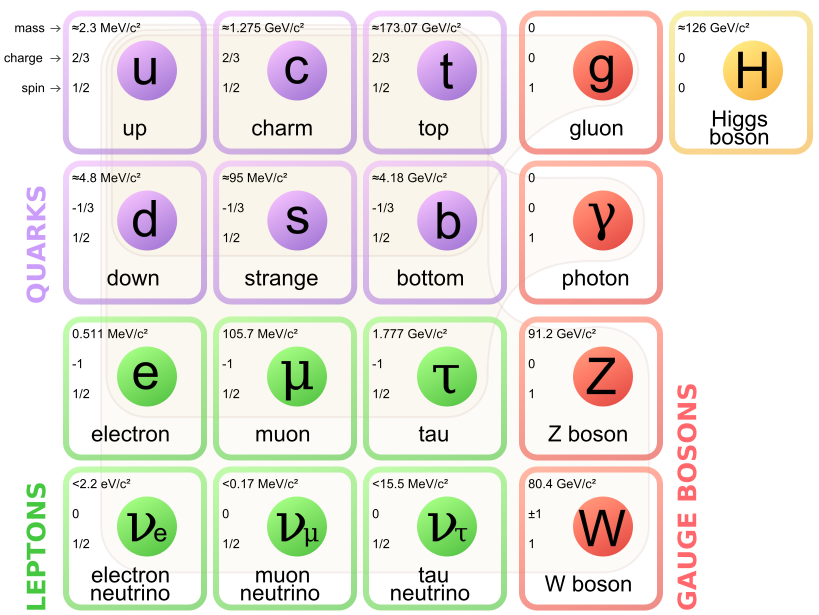
\includegraphics[width=0.7\textwidth]{figures/SM}
 \let\thefootnote\relax\footnotetext{Image courtesy of PBS Nova.}
\end{frame}

\subsection*{What is a muon?}

\begin{frame}{What is a muon?}{Introduction to Muon Physics}
  \begin{block}{Discovery}
Discovered by Carl Anderson and Seth Neddermeyer at Caltech (California, USA) in 1936. 
\end{block}
\begin{block}{Properties}
Spin-\nicefrac{1}{2}, charge -$e$; 200 times heavier than an electron. Lifetime is $\sim$ 2.19 $\mu s$ in vacuum.\\
Muons are \textbf{natural} by-products of cosmic rays.
Can also be produced \textbf{artificially} in the laboratory (same principle as with cosmic rays). 
\end{block}

\begin{itemize}
\item $\sim$ 200 \textbf{cosmic} muons reach every $m^2$ per second. 
\item Travel up to 20 $km$ in the atmosphere thanks to Relativity, as opposed to 660 m. 
\item Penetrate metres into the ground and eventually captured on atoms (N.B. muon tomography in pyramids!). 
\end{itemize}
  
\end{frame}

\begin{frame}{Why muon?}{Introduction to Muon Physics}


\begin{itemize}
\item Heavier mass than electron.
\item Relatively long lifetime - longest of all unstable elementary particles!
\item Extremely Penetrating.
\end{itemize}

\begin{equation}
\mu^- \rightarrow e^- + \bar{\nu_{e}} + \nu_{\mu},
\label{eq:mu-_int}
\end{equation}

\begin{figure}
\centering
\begin{minipage}{.4\textwidth}
\centering
\begin{fmffile}{simple_tree_1}
\setlength{\unitlength}{0.12cm}
\begin{fmfgraph*}(40,35)
\fmfleft{i}
\fmfright{o1,o2,o3}
\fmf{fermion, label=$\mu^-$}{i,v1}
\fmf{fermion, label=$\nu_{\mu}$, label.side=left}{v1,o1}
\fmf{boson, label=$W^-$,tension=.7}{v1,v2}
%\fmf{fermion, label=$e^-$, label=$\nu_e$}{o2,v2,o3}
\fmf{fermion, label=$\bar{\nu_e}$}{o2,v2}
\fmf{fermion, label=$e^-$}{v2,o3}
\end{fmfgraph*}
\end{fmffile}
%\caption{A subfigure}
\end{minipage}
%\caption{A figure with two subfigures}
\end{figure}
\end{frame}

% \begin{frame}{Why muon?}{Introduction to Muon Physics}
% The energy loss of a charged particle is described by the Bethe-Barkas-Andersen-Bloch formula:
% \begin{equation}
% - \left\langle\frac{dE}{dx}\right\rangle = \frac{4 \pi}{m_e c^2} \cdot \frac{nz^2}{\beta^2} \cdot \left(\frac{e^2}{4\pi\varepsilon_0}\right)^2 \cdot \left[\ln \left(\frac{2m_e c^2 \beta^2}{I \cdot (1-\beta^2)}\right) - \beta^2\right]
% \end{equation}
% For muons with $\sim$ 100 MeV to 100 GeV the ionisation losses dominate:
%\end{frame}

\begin{frame}{Muon Experiments}{Introduction to Muon Physics}
Some of the past, present and future muon physics experiments [1]. 
\Fontvi
\begin{itemize}
    \item Muon lifetime: MuLan, FAST - strength of the weak interaction (through the Fermi constant, $G_F$).
    \item Muon decay: TWIST - asymmetry of weak interactions. 
\item Charged Lepton Flavor Violation (cLFV): Mu2e, Mu3e, COMET - precision tests of the Standard Model (SM).
\item Dipole Moments:  Brookhaven g-2 (E821), \textbf{Fermilab g-2 (E989)}, J-PARC g-2 - looking for signs of physics Beyond the Standard Model (BSM), and sources of charge-parity (CP) violation. 
\item Nuclear muon capture: MuCap, \textbf{MuSun}, AlCap  - precision tests of nuclear reactions.  
\item Muonium ($\mu^+e^-$) bound states: LAMPF, MuSEUM - investigation of hydrogen-like \textit{leptonic} \say{atoms}.   
\item Muonic Lamb shift: - measurement of the proton radius. \\
\end{itemize}

Muon spin spectroscopy, muon tomography, etc. 
\let\thefootnote\relax\footnotetext{\textit{Precision Muon Physics}, T. Gorringe, D. Hertzog}
\end{frame}

%%%%%%%%%%%%%%%%%%%%%%%%%%%%%%%%%%%%%%%%%%%%%%%%%%%%%%%%%%%%%%%%%
\section{Overview of MuSun experiment}

\subsection{Introduction to the Paul Scherrer Institute (PSI)}

\begin{frame}{Location: Paul Scherrer Institute (PSI)}{MuSun}
 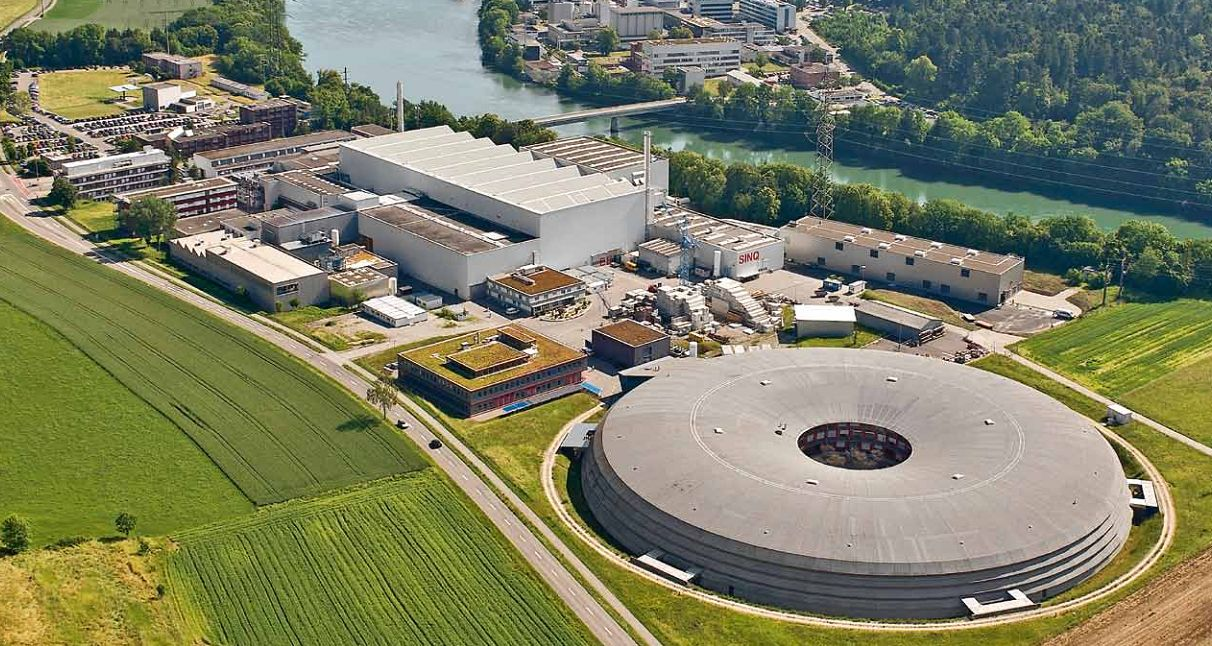
\includegraphics[width=\textwidth]{figures/psi.jpg}
 \let\thefootnote\relax\footnotetext{Image courtesy of PSI.}
\end{frame}



\begin{frame}{Experimental Beamlines at PSI}{MuSun}
 \begin{columns}[onlytextwidth]
  \begin{column}{0.4\textwidth}
  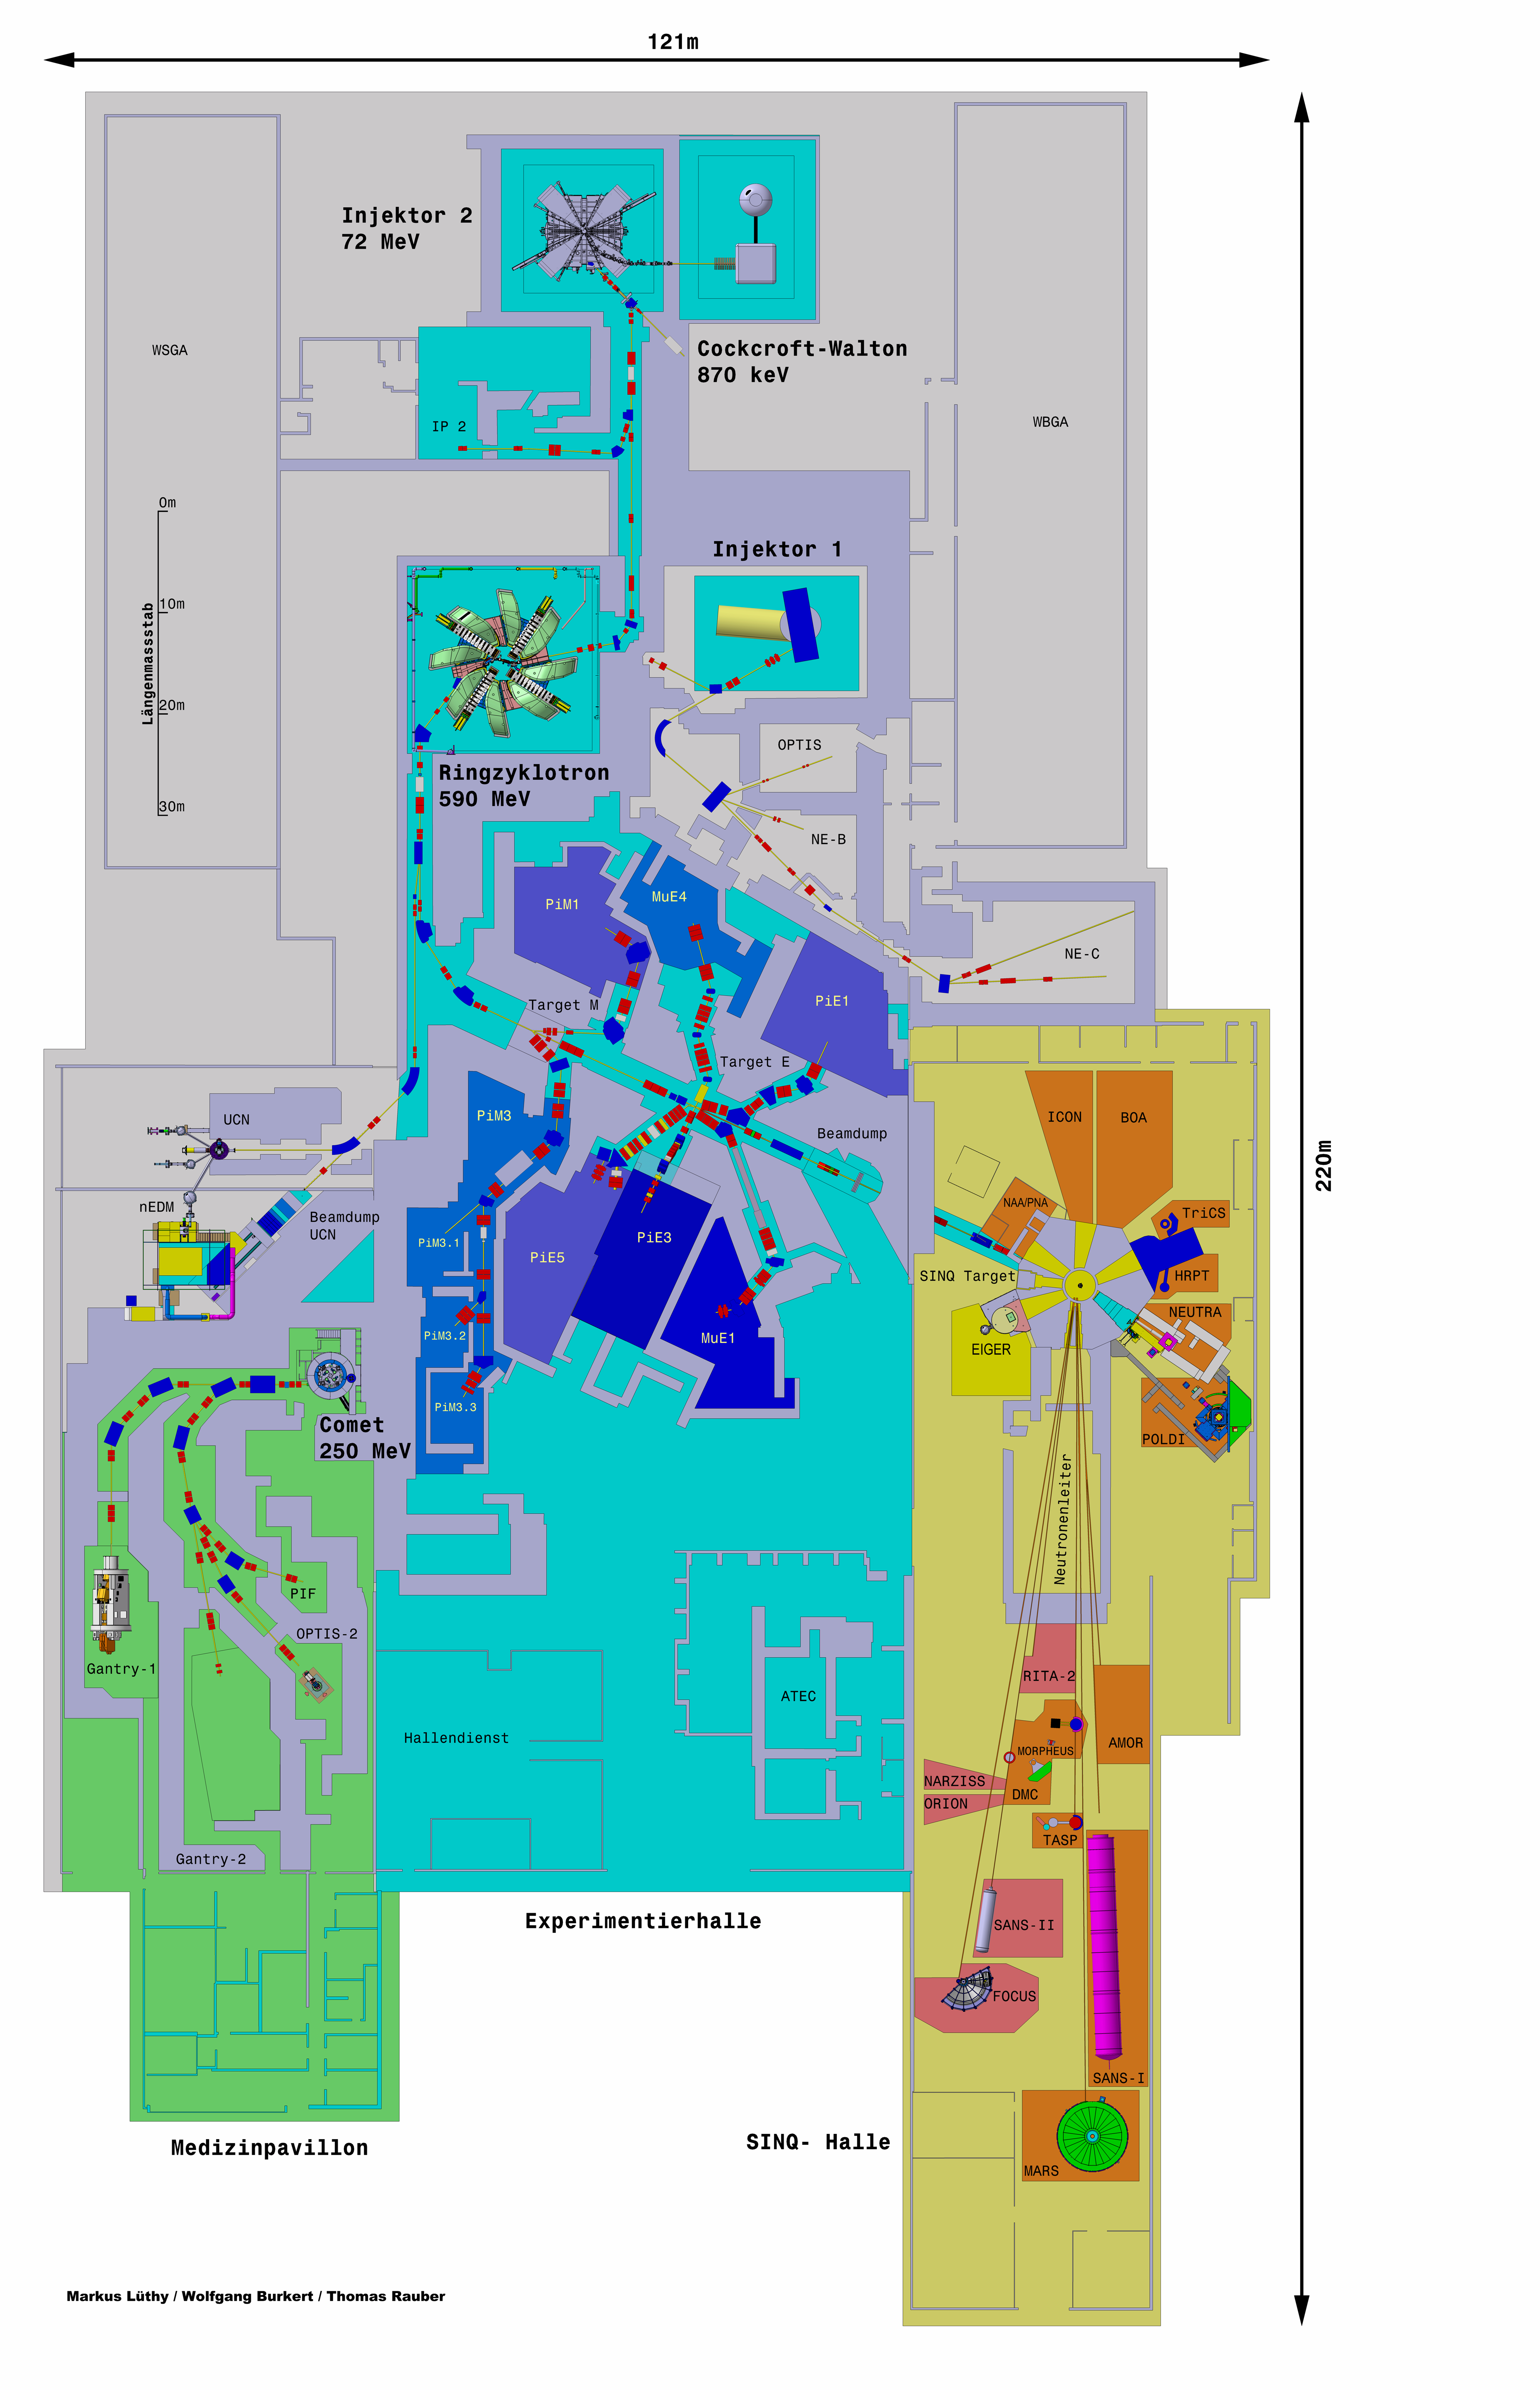
\includegraphics[height=0.8\textheight]{figures/HallenplanPSI.png} \\
  \end{column}
  \begin{column}{0.25\textwidth}
  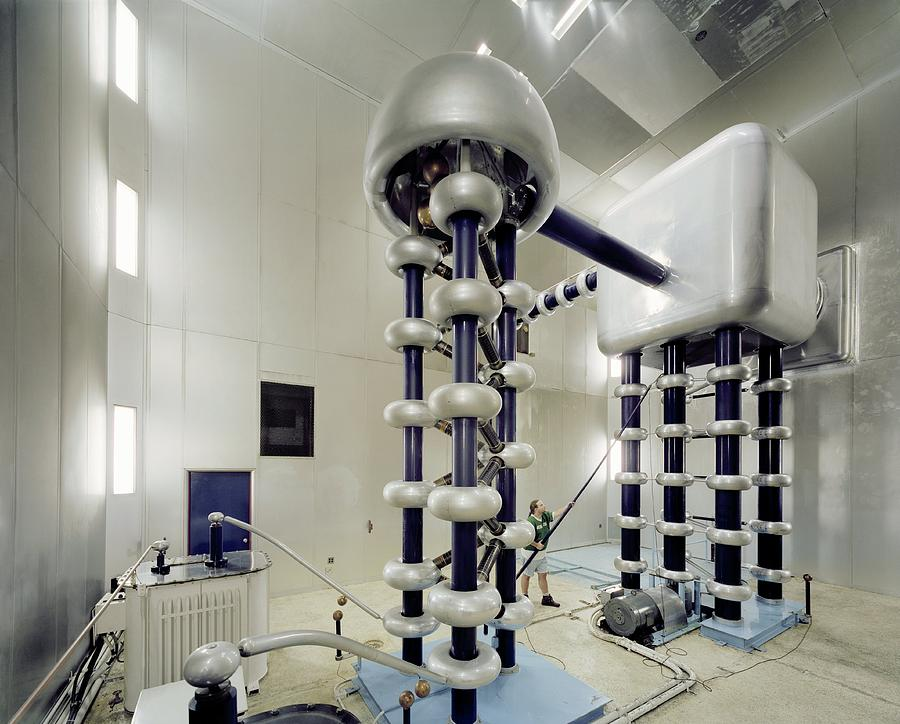
\includegraphics[height=0.25\textheight]{figures/cw.jpg} \\
  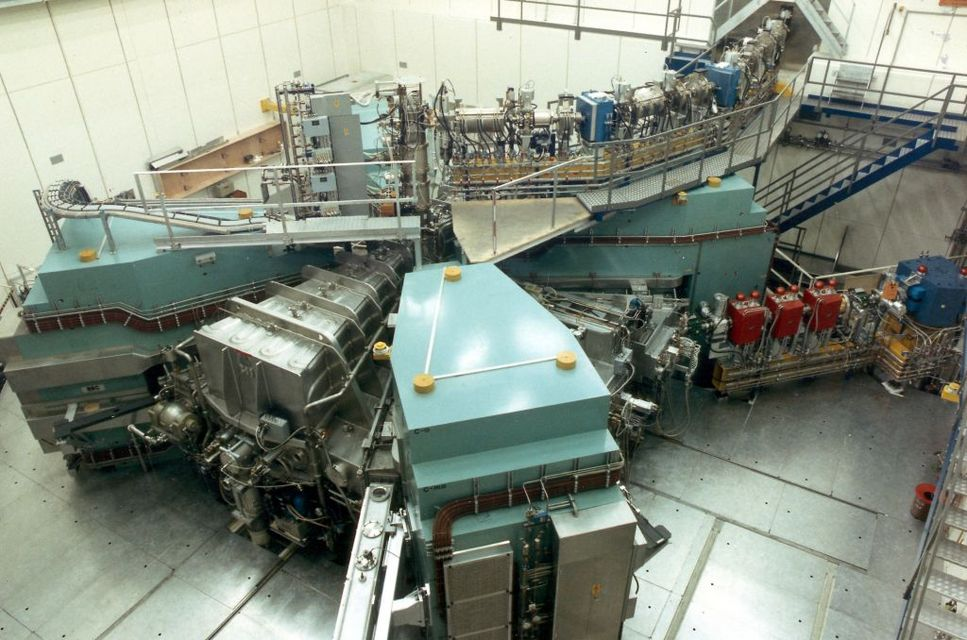
\includegraphics[height=0.25\textheight, trim=0 0 1.4cm 0, clip]{figures/inj.jpg} \\
 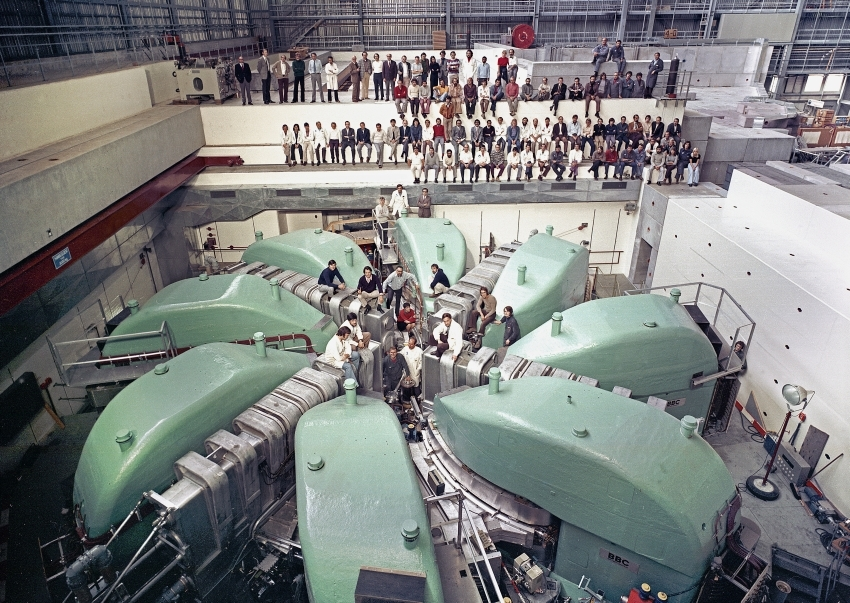
\includegraphics[height=0.25\textheight, trim=0 0 2.95cm 0, clip]{figures/rz.jpg}\\
  \end{column}
   \begin{column}{0.3\textwidth}
   \normalsize{\textbf{Proton Acceleration:} \\Ion source: 60 keV \\ $\downarrow$\\ Cockcroft-Walton\\ accelerator: 870 keV \\ $\downarrow$ \\ Injector-II: 72 MeV \\ $\downarrow$ \\ Ring Cyclotron: \\ 590 MeV, 2.2 mA}
   \end{column}
  \end{columns}
  \let\thefootnote\relax\footnotetext{Images courtesy of PSI.}
\end{frame}

\begin{frame}{Muon Beam at PSI}{MuSun}
\Fontvi
The source of muons ($\mu^+$ or $\mu^-$) are pions, which are produced by sending a (590 MeV) proton beam on a (graphite) target:  
\begin{equation}
p ~(590 MeV) + p ~(target) \rightarrow p + n + \boldsymbol{\pi^+},
\end{equation}
or 
\begin{equation}
p ~(590 MeV) + n ~(target) \rightarrow p + p + \boldsymbol{\pi^-},
\end{equation}

The pions subsequently decay into muons:
\begin{equation}
\pi^+ \rightarrow \mu^+ + \nu_{\mu},
\end{equation}
and
\begin{equation}
\pi^- \rightarrow \mu^- + \bar{\nu_{\mu}}.
\end{equation}

The muons will then decay
\begin{equation}
\mu^+ \rightarrow e^+ + \nu_{e} + \bar{\nu_{\mu}},
\label{eq:mu+}
\end{equation}
and
\begin{equation}
\mu^- \rightarrow e^- + \bar{\nu_{e}} + \nu_{\mu},
\label{eq:mu-}
\end{equation}

\end{frame}


\begin{frame}{The Main Control Room at PSI}{MuSun}
  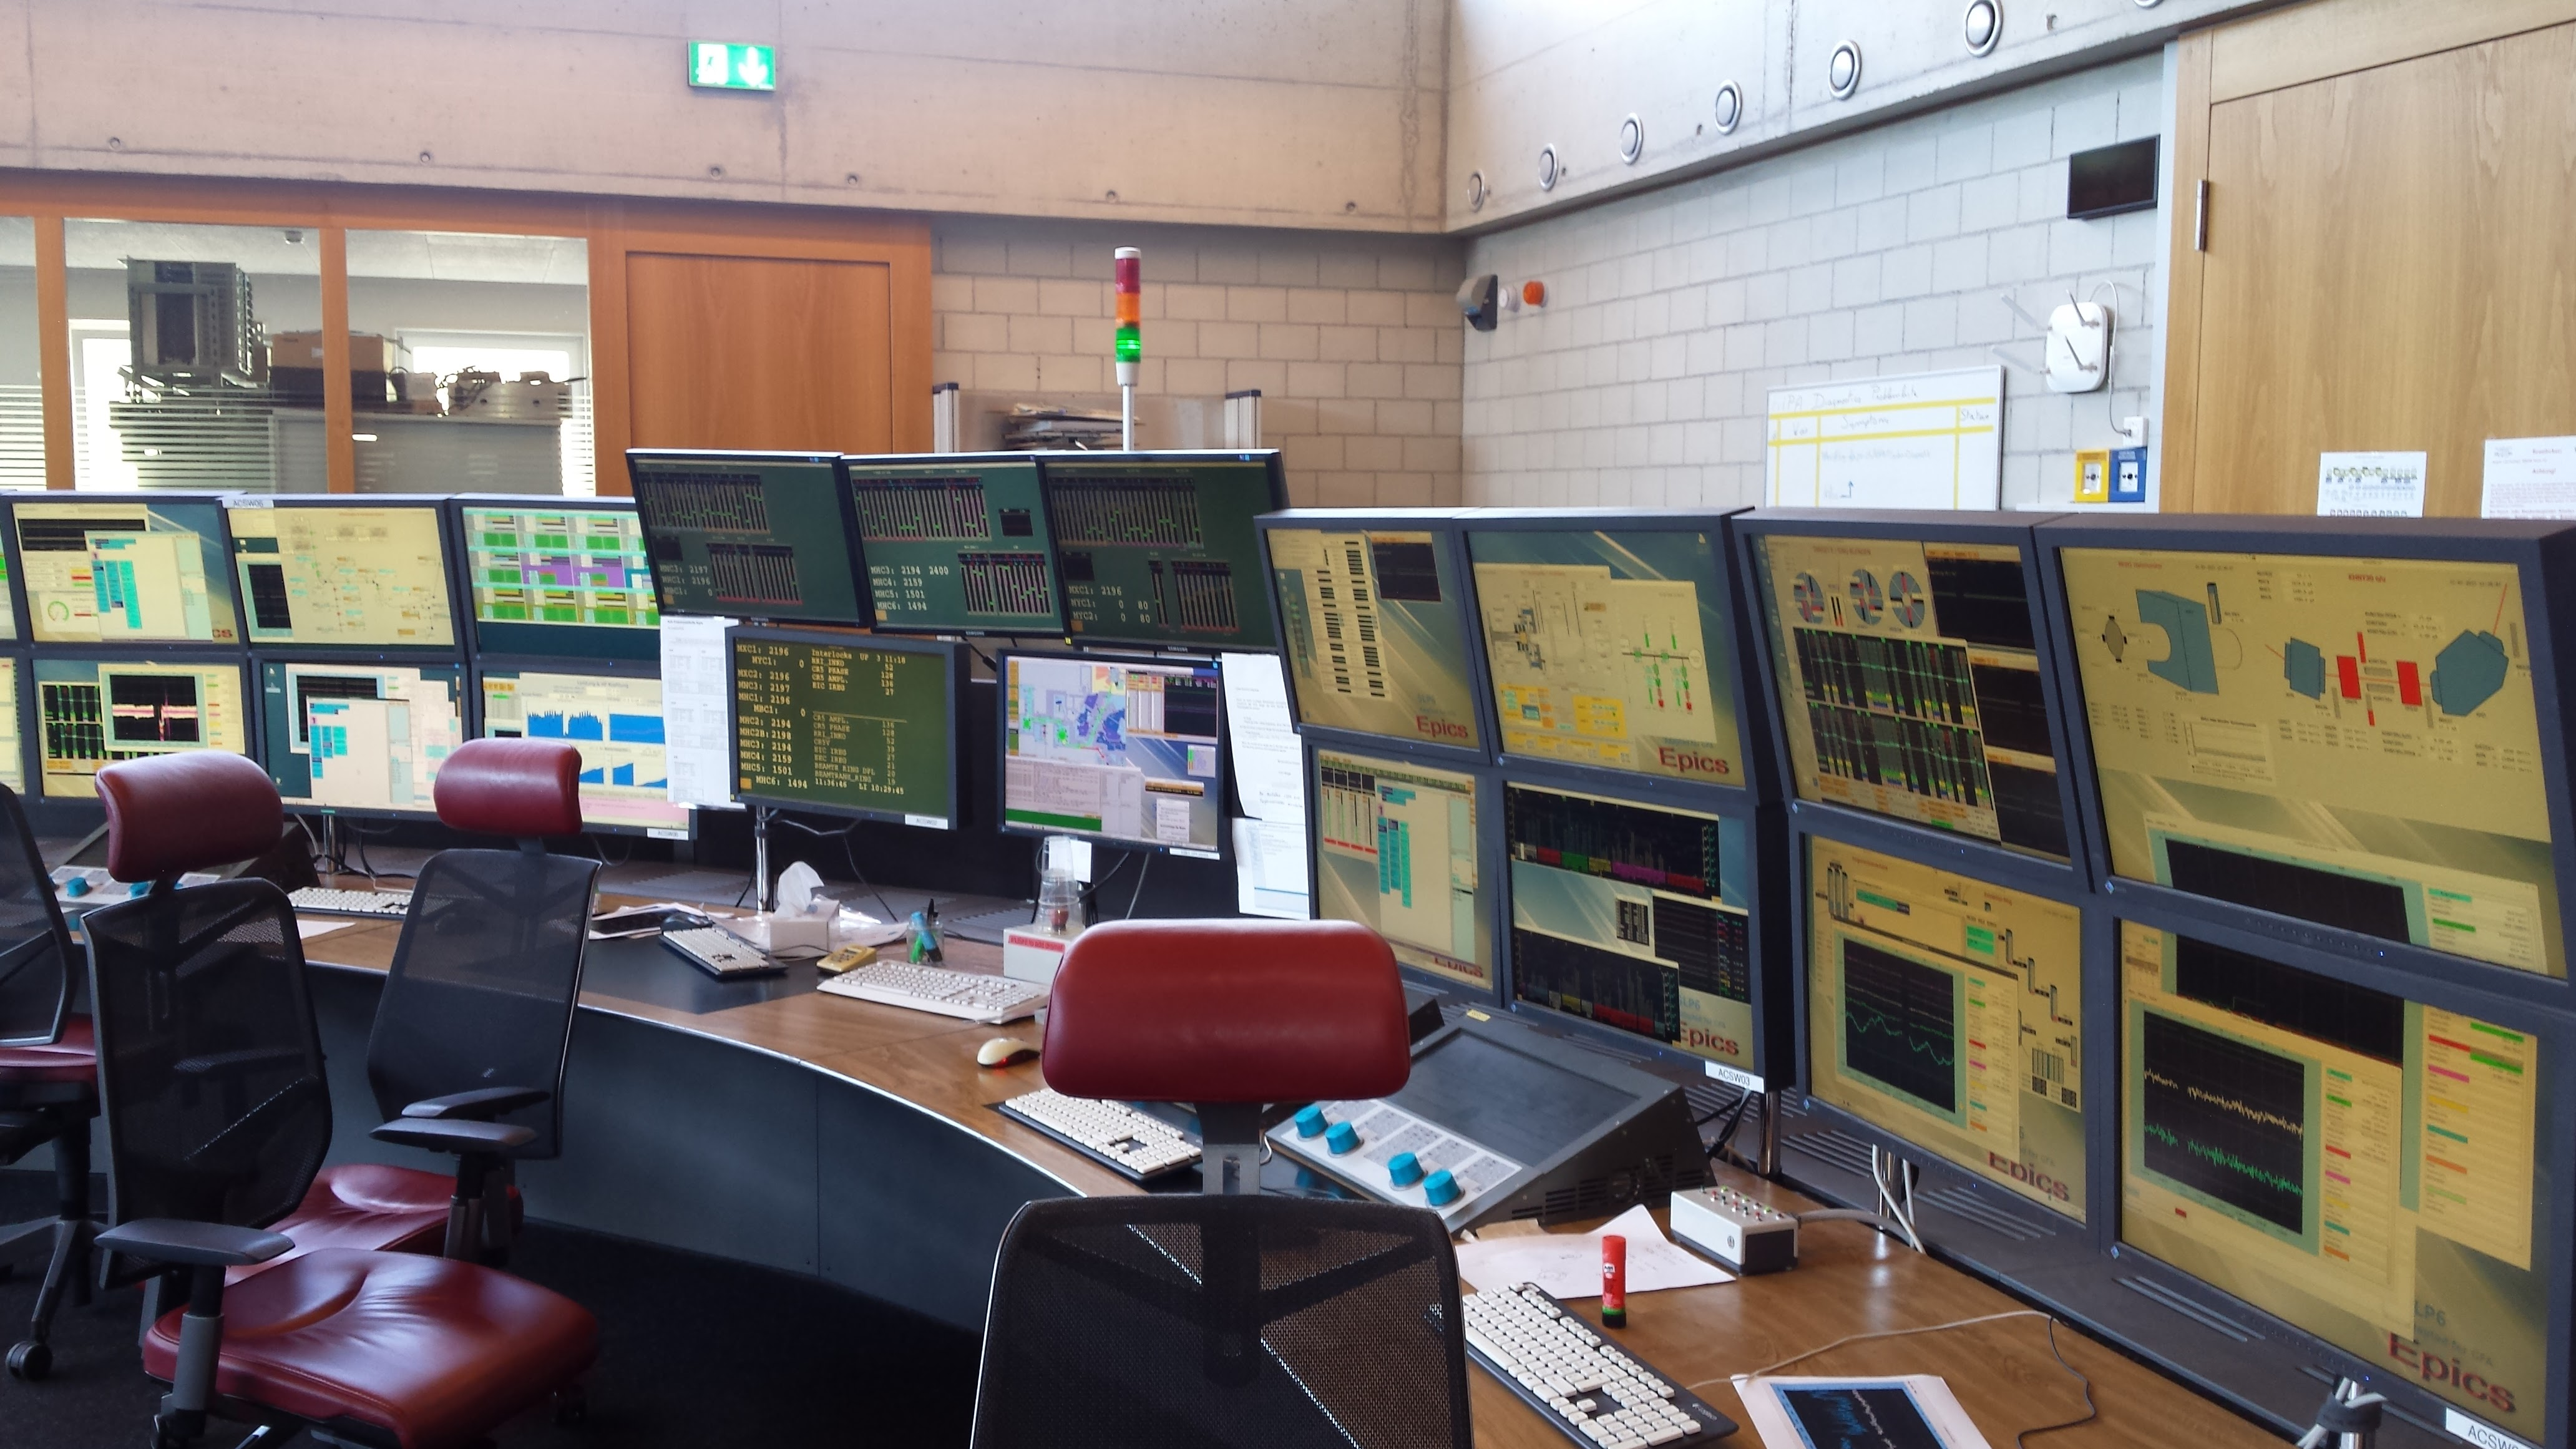
\includegraphics[width=\textwidth]{figures/control_room.jpg}\\
\end{frame}

\begin{frame}{The Experimental Hall at PSI}{MuSun}
  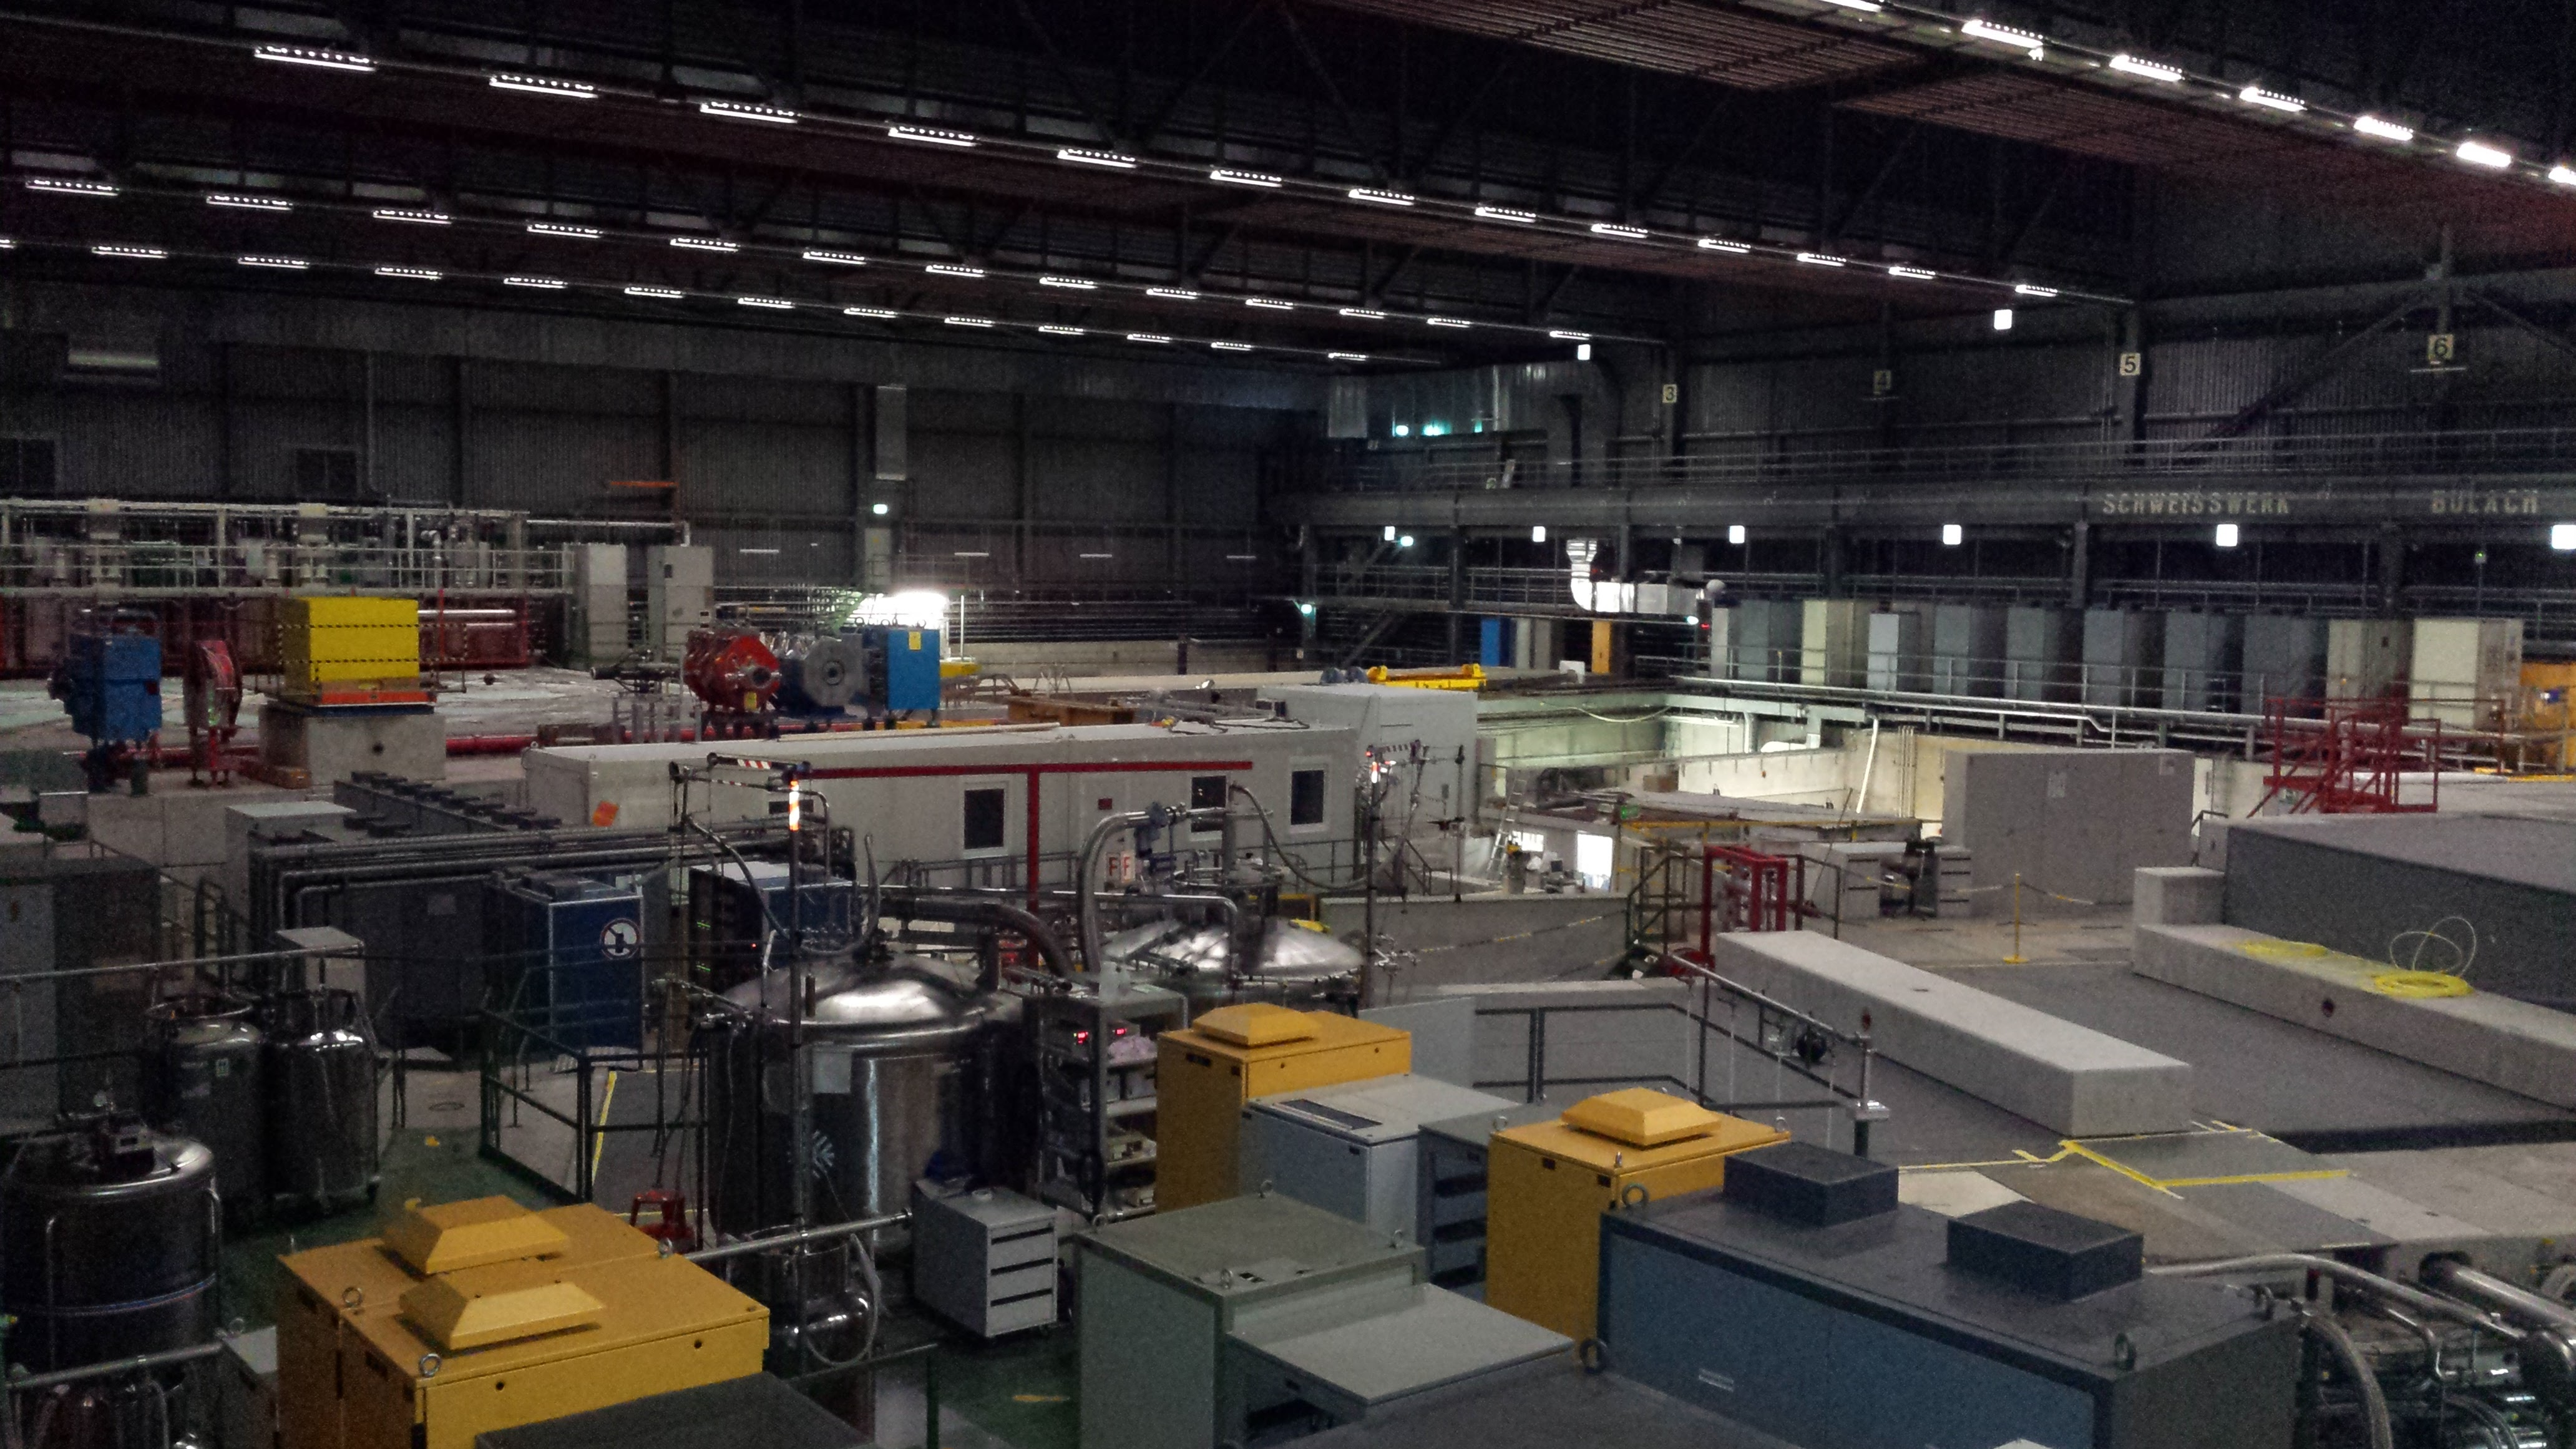
\includegraphics[width=\textwidth]{figures/hall.jpg}\\
\end{frame}

\begin{frame}{The Experimental Hall at PSI}{MuSun}
  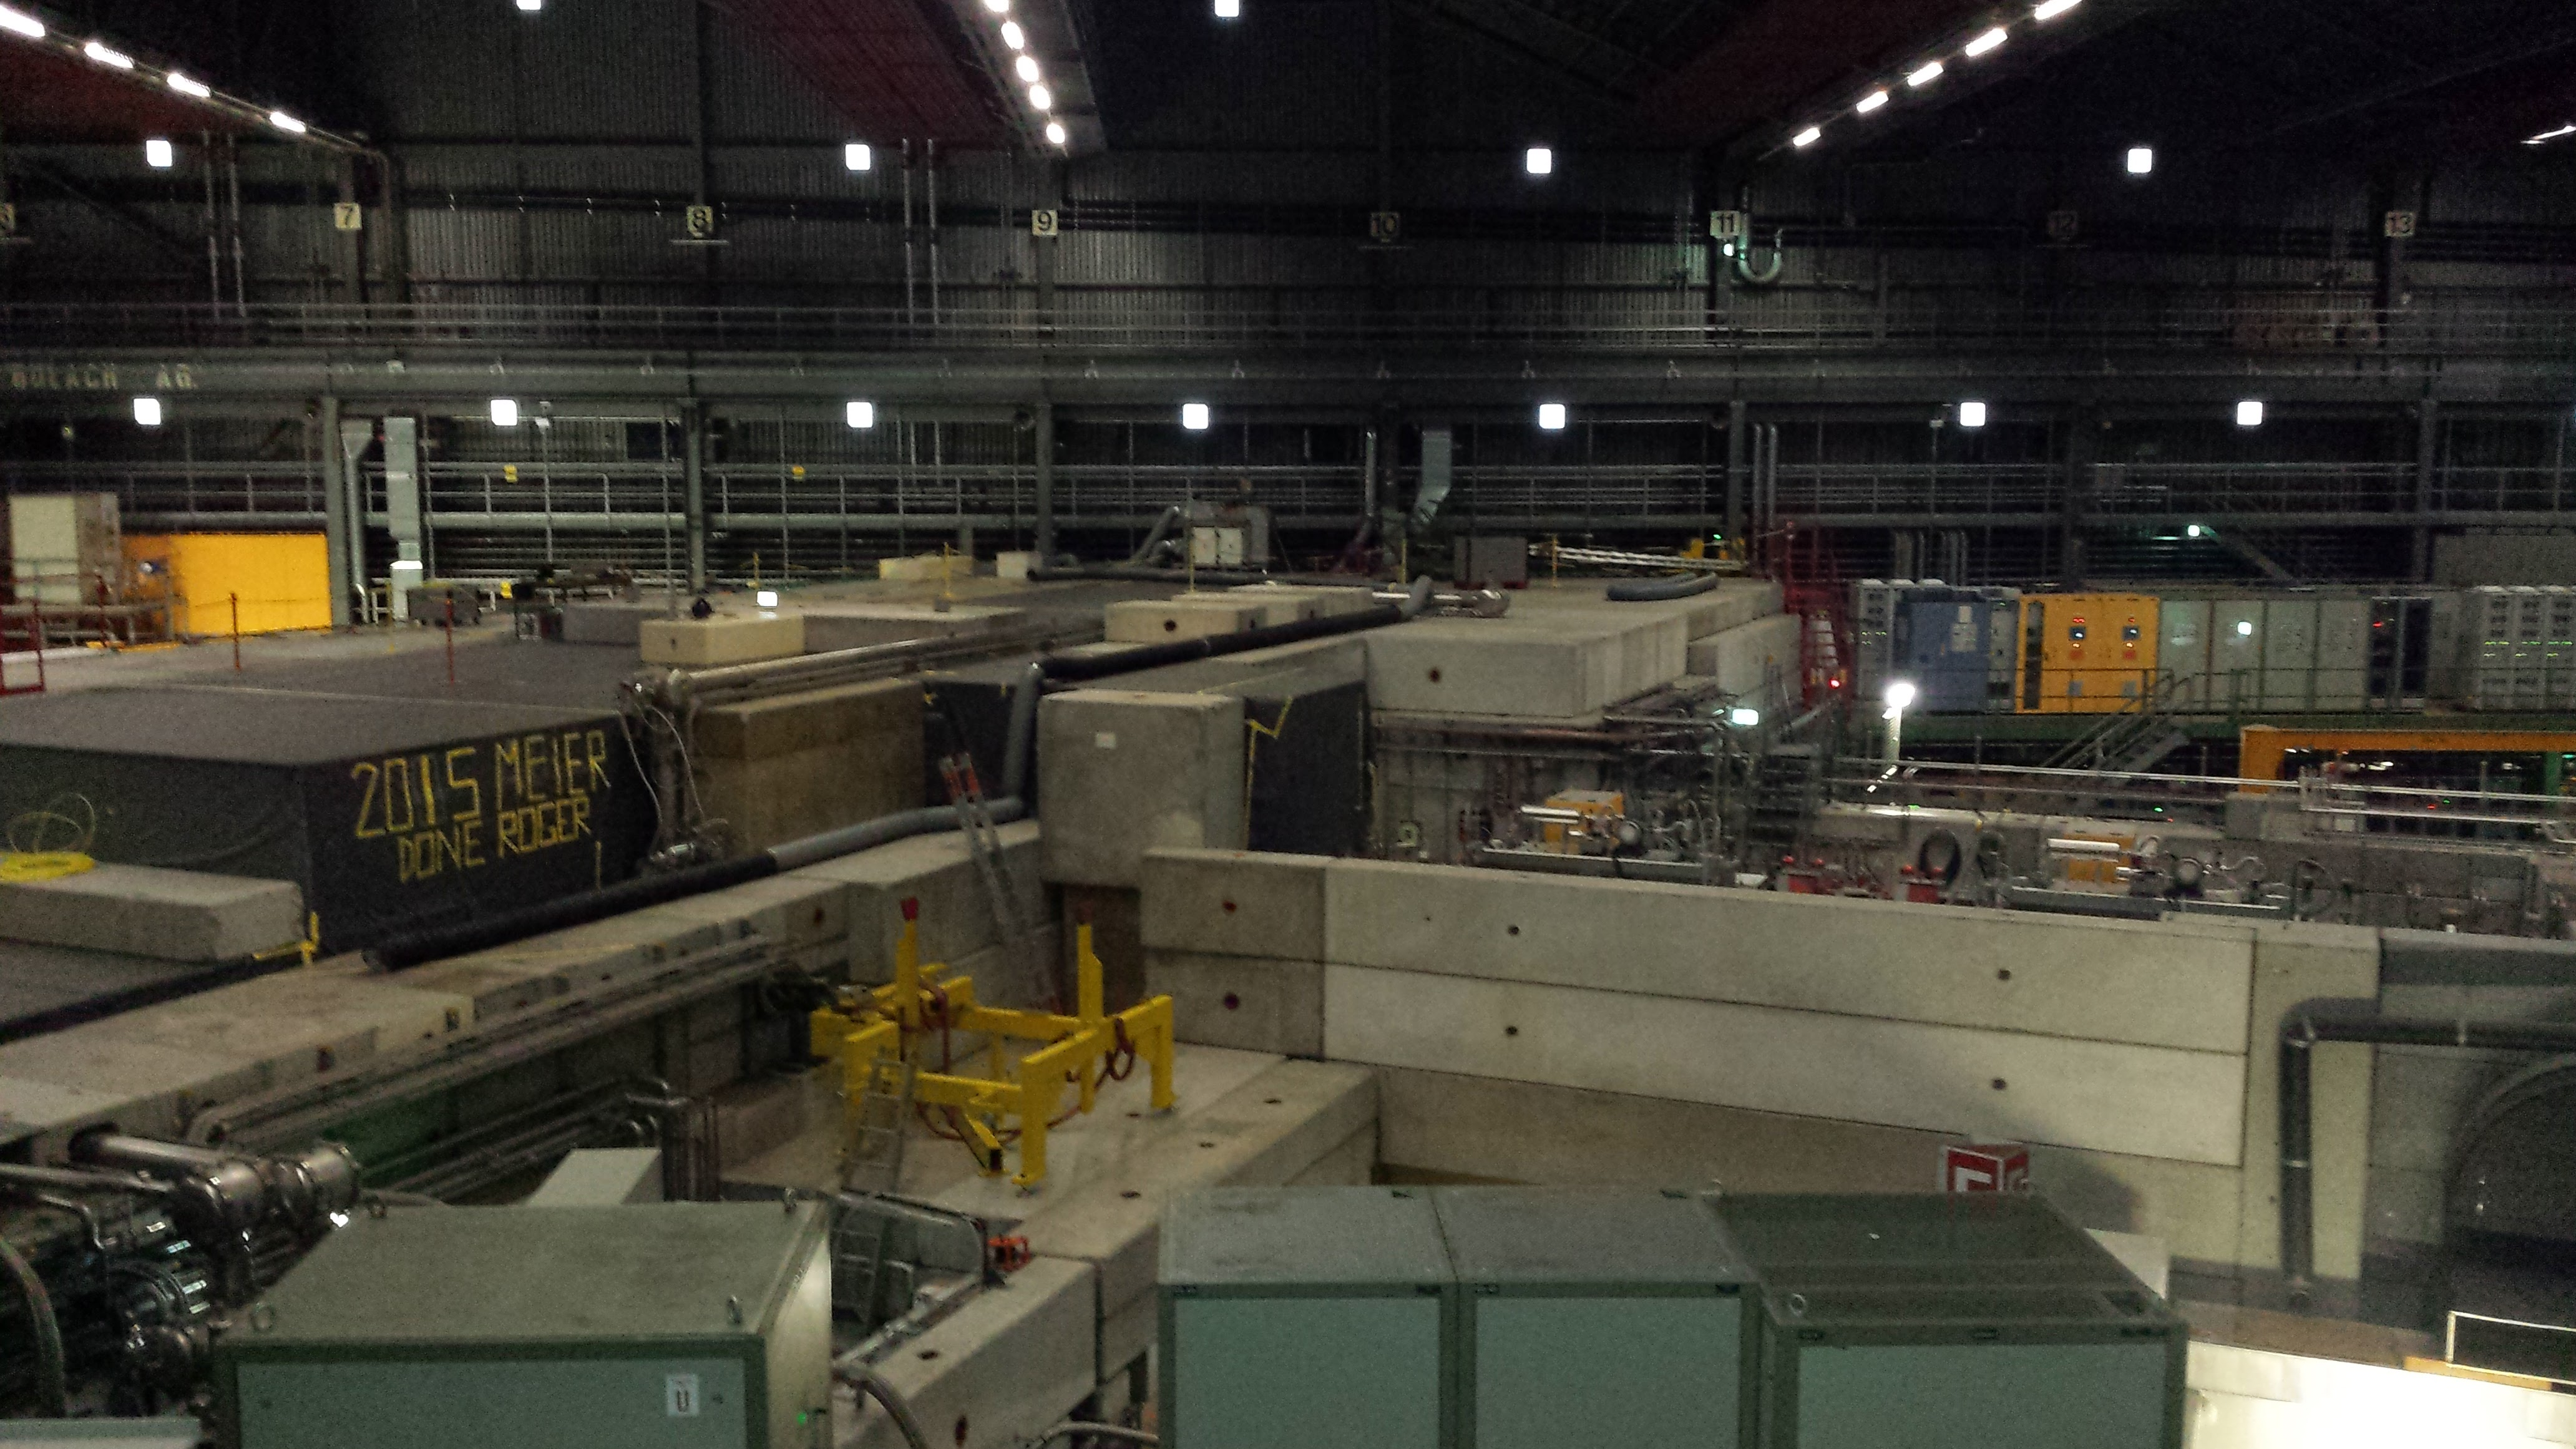
\includegraphics[width=\textwidth]{figures/hall_2.jpg}\\
\end{frame}

\begin{frame}{The Beamline}{MuSun}
  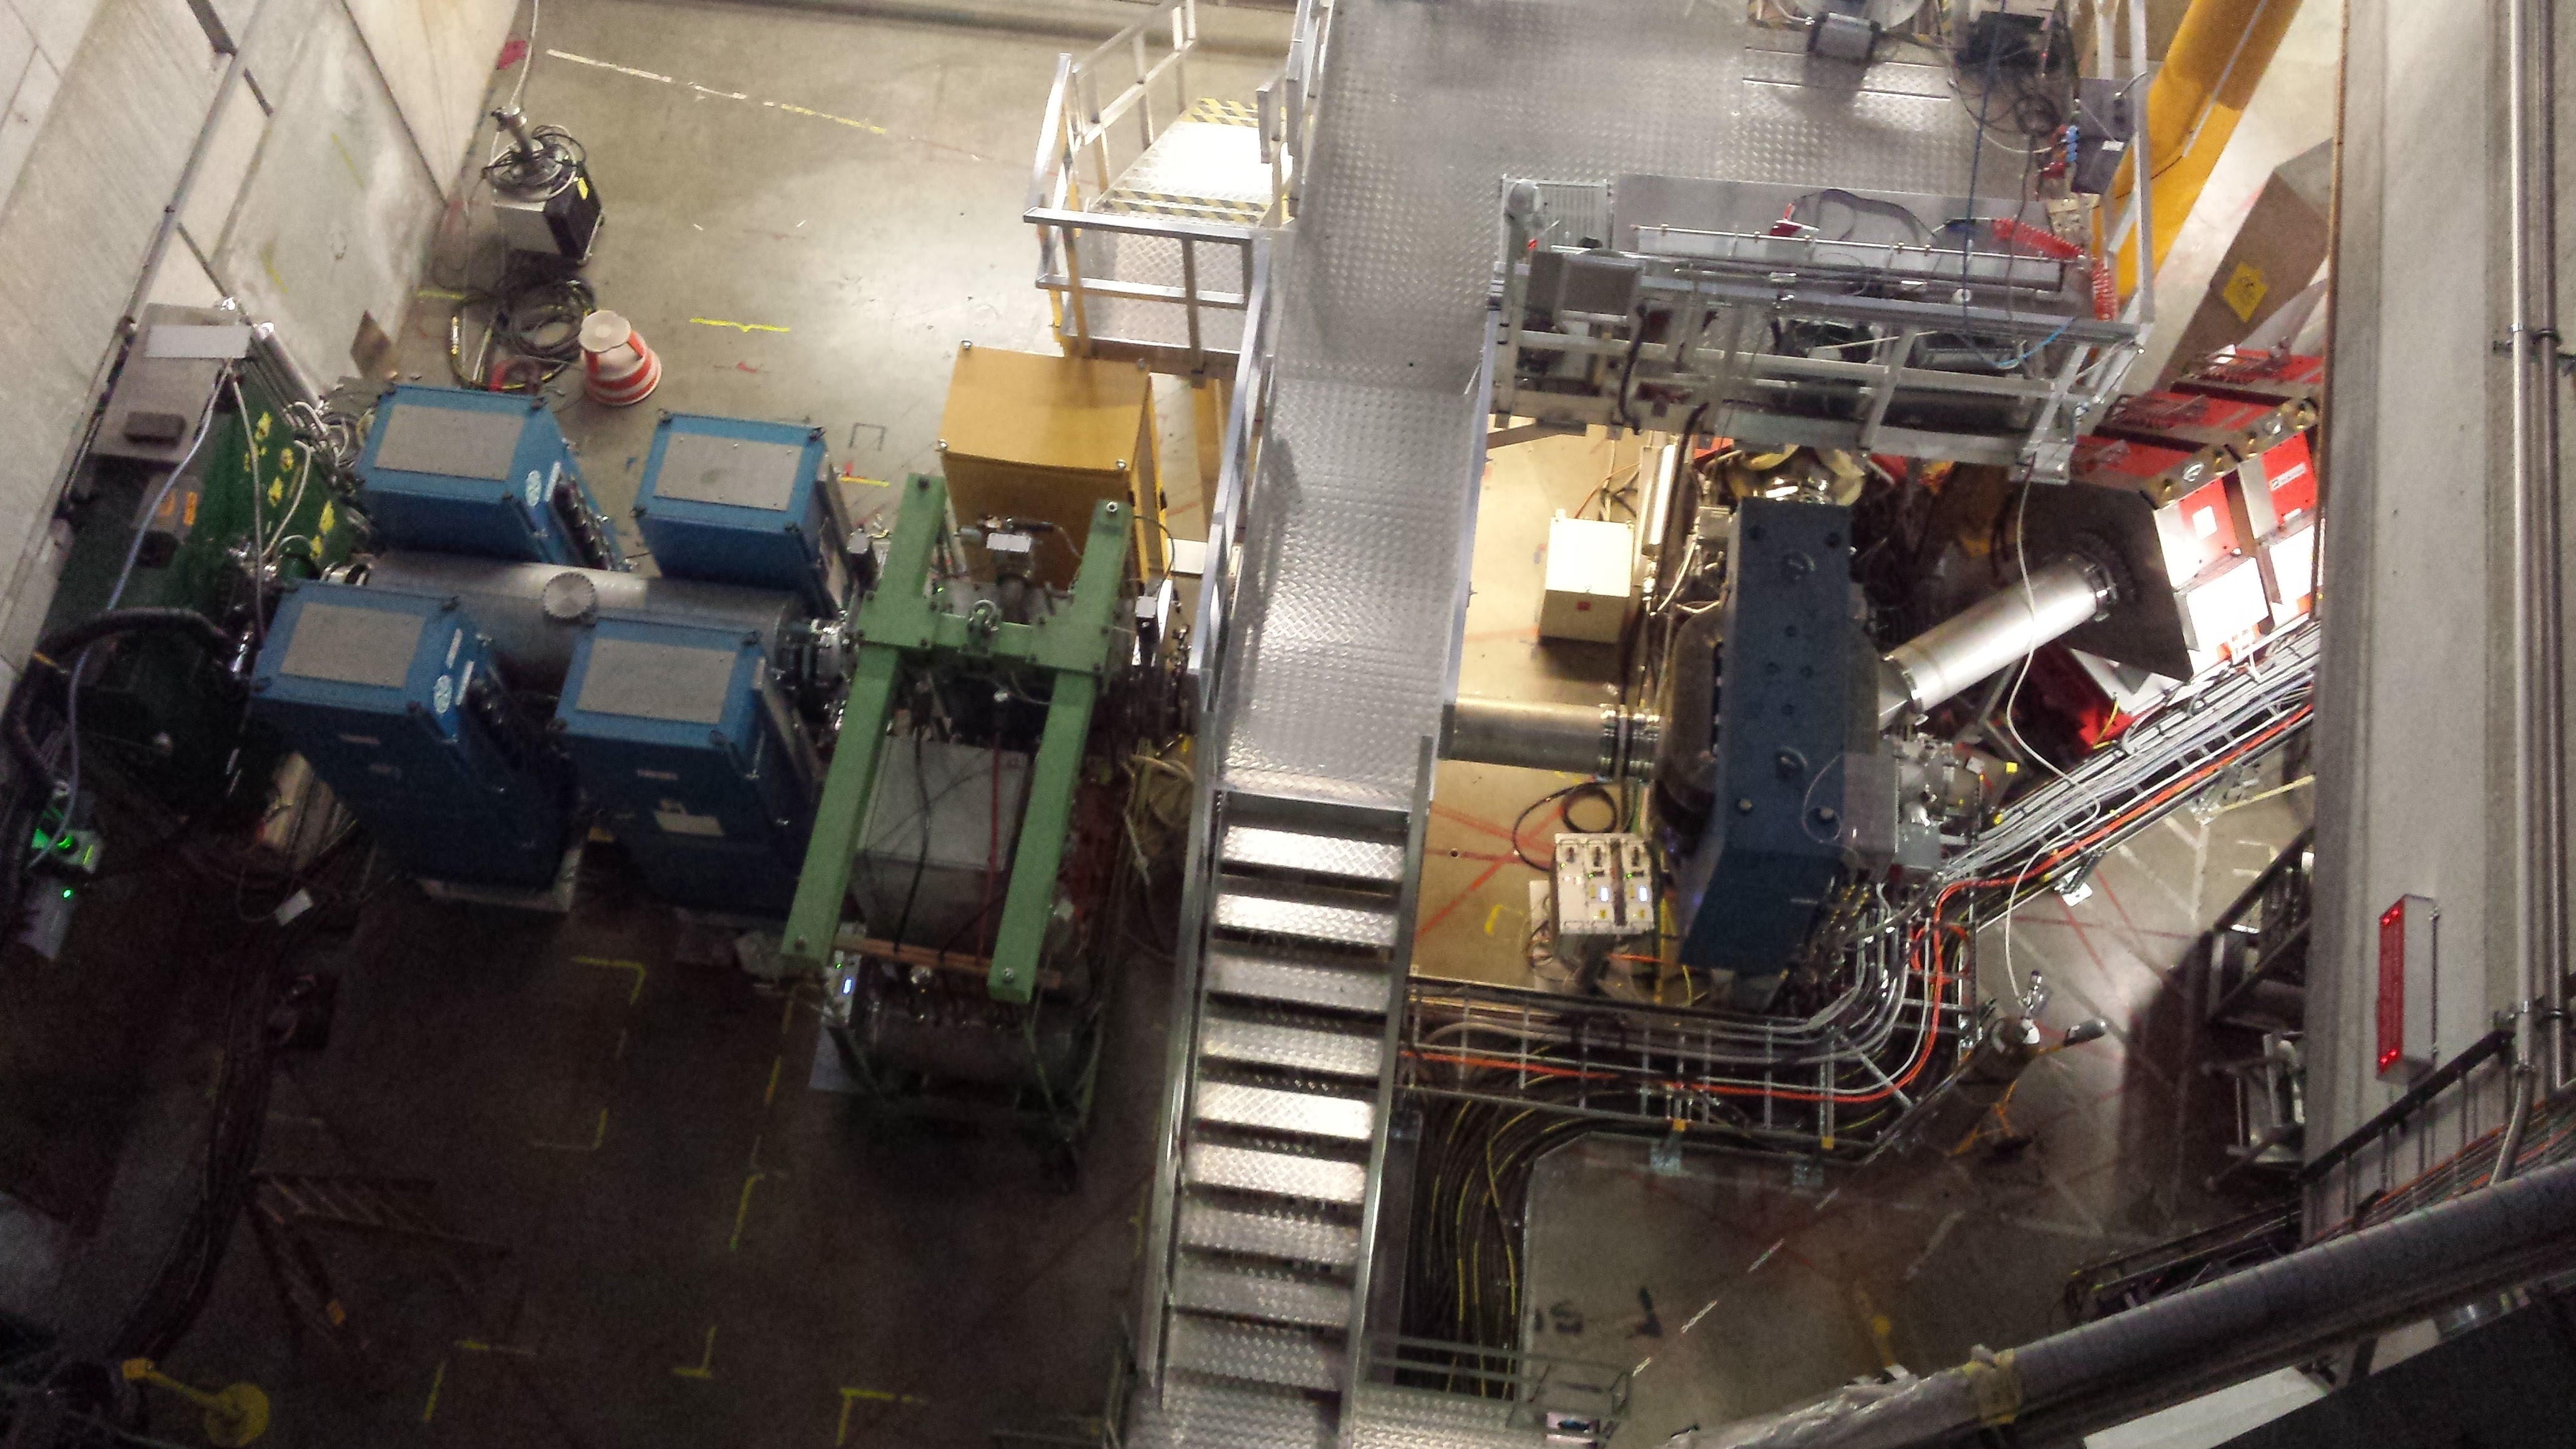
\includegraphics[width=\textwidth]{figures/beamline.jpg} \\
\end{frame}


\subsection{Experimental Techniques and Apparatus}

\begin{frame}{Aim}{MuSun}
  \begin{block}{Aim}
To measure the muon lifetime on deuterium to a 1.5\% precision.  
     \end{block}
  
  \begin{block}{Properties of deuterium.}
${_{1}^{2}H}$ is just an \textit{isotope} of hydrogen. However, an extremely pure gas of ppb (parts per billion) purity is required for the experiment! 
\end{block}

\begin{figure}
\centering
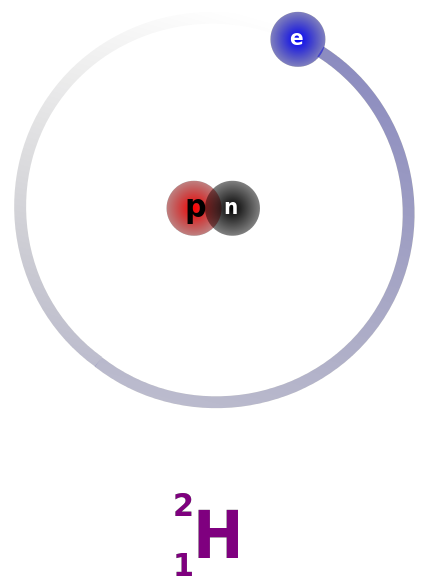
\includegraphics[height=0.3\textheight]{figures/h.png}
\let\thefootnote\relax\footnotetext{Image courtesy of Dirk Hunniger.}
\label{fig:my_label}
\end{figure}

\end{frame}

% You can reveal the parts of a slide one at a time

% with the \pause command:
\begin{frame}{Why capturing a muon on deuterium?}{MuSun}
  \begin{itemize}
  \item {Creating \textbf{muonic} atoms.}
  \item {Measurement ($7 \times 10^9$ events collected in summer 2015): 
  \begin{equation}
  \Lambda _d=\lambda_- - \lambda_+    
  \end{equation}
  \begin{equation}
  \mu^- + {_{1}^{2}H^+} \rightarrow n + n + \nu_{\mu} 
  \end{equation} }
  \item The simplest (weak force) reaction on a nucleus that can be both measured \textit{experimentally} and estimated \textit{theoretically}
  \item Will help to \say{scale} models (e.g. EFT, QCD) and guide theorists.
  \end{itemize}
 
 \begin{block}{Solar connection}
  \say{Calibrating the Sun}: hence the name! 
  Understating the astrophysical reactions (e.g. proton fusion: $p + p \rightarrow  {_{1}^{2}H^+} + e^+ + \nu_{e} $) powering the Sun!
\end{block}
 
\end{frame}

\begin{frame}{The Detectors}{MuSun}
\centering
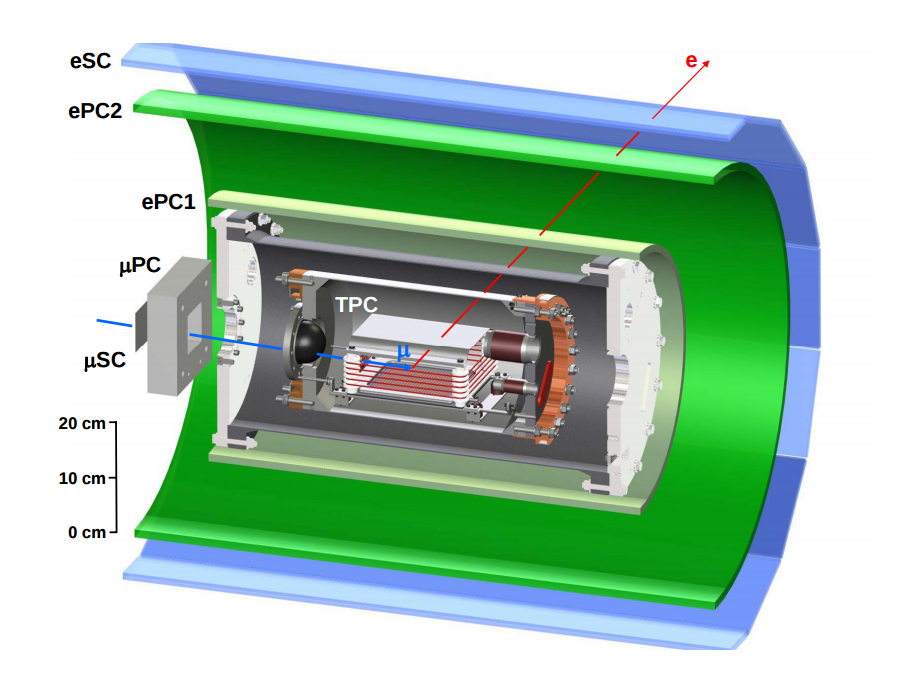
\includegraphics[width=0.8\textwidth]{figures/tpc.png}
\let\thefootnote\relax\footnotetext{Image courtesy of the MuSun Collaboration [2].}
\end{frame}
\begin{frame}{The Detectors}{MuSun}
\centering
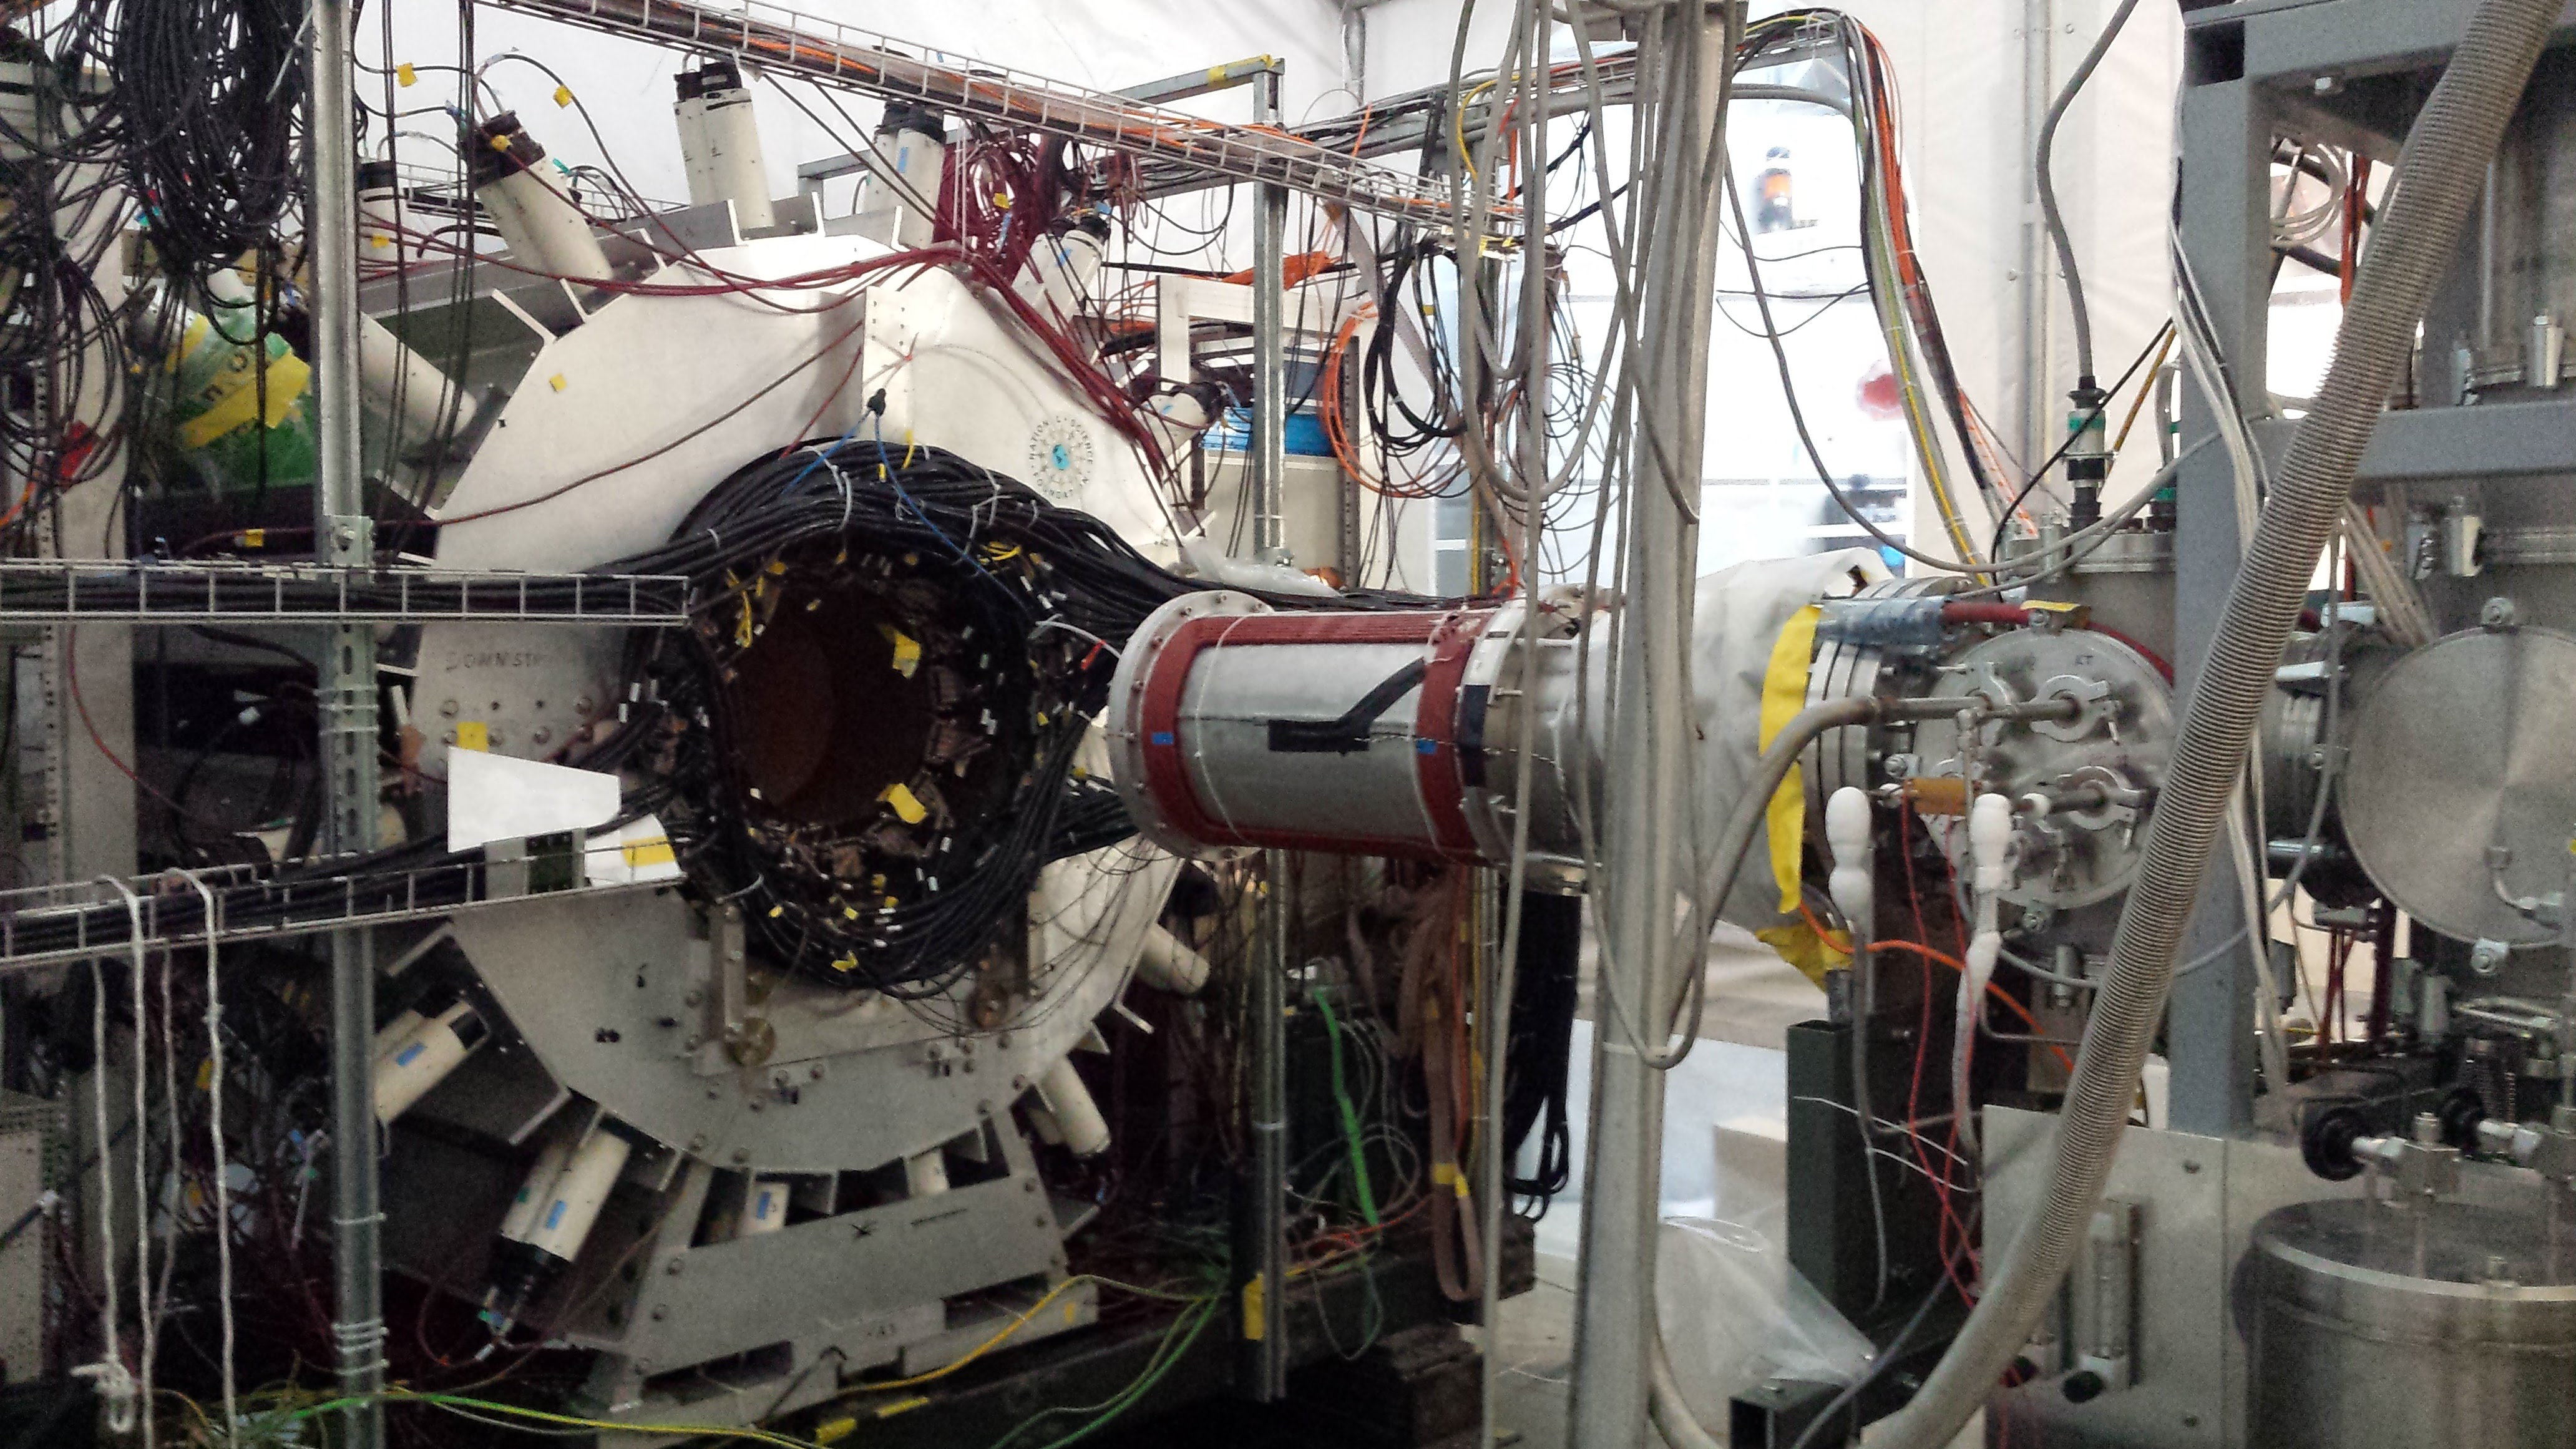
\includegraphics[width=\textwidth]{figures/tpc.jpg}
\end{frame}


\begin{frame}{The Detectors}{MuSun}
\centering
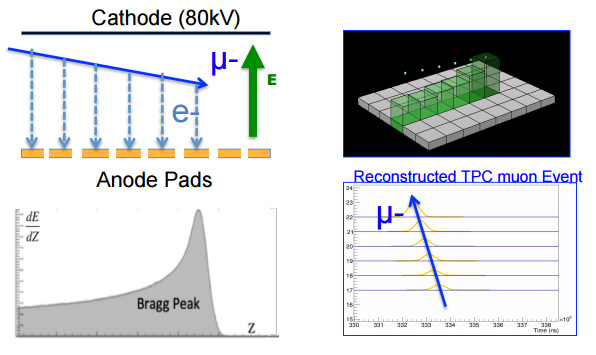
\includegraphics[width=0.8\textwidth]{figures/tpc_2.png}
\let\thefootnote\relax\footnotetext{Image courtesy of the MuSun Collaboration [2].}
\end{frame}

\begin{frame}{The DAQ}{MuSun}
  \begin{itemize}
  \item {
   Data flow: 0.64 TB per day of data. 
   
   That is equivalent to 140 DVD disks worth of data! 
  }
  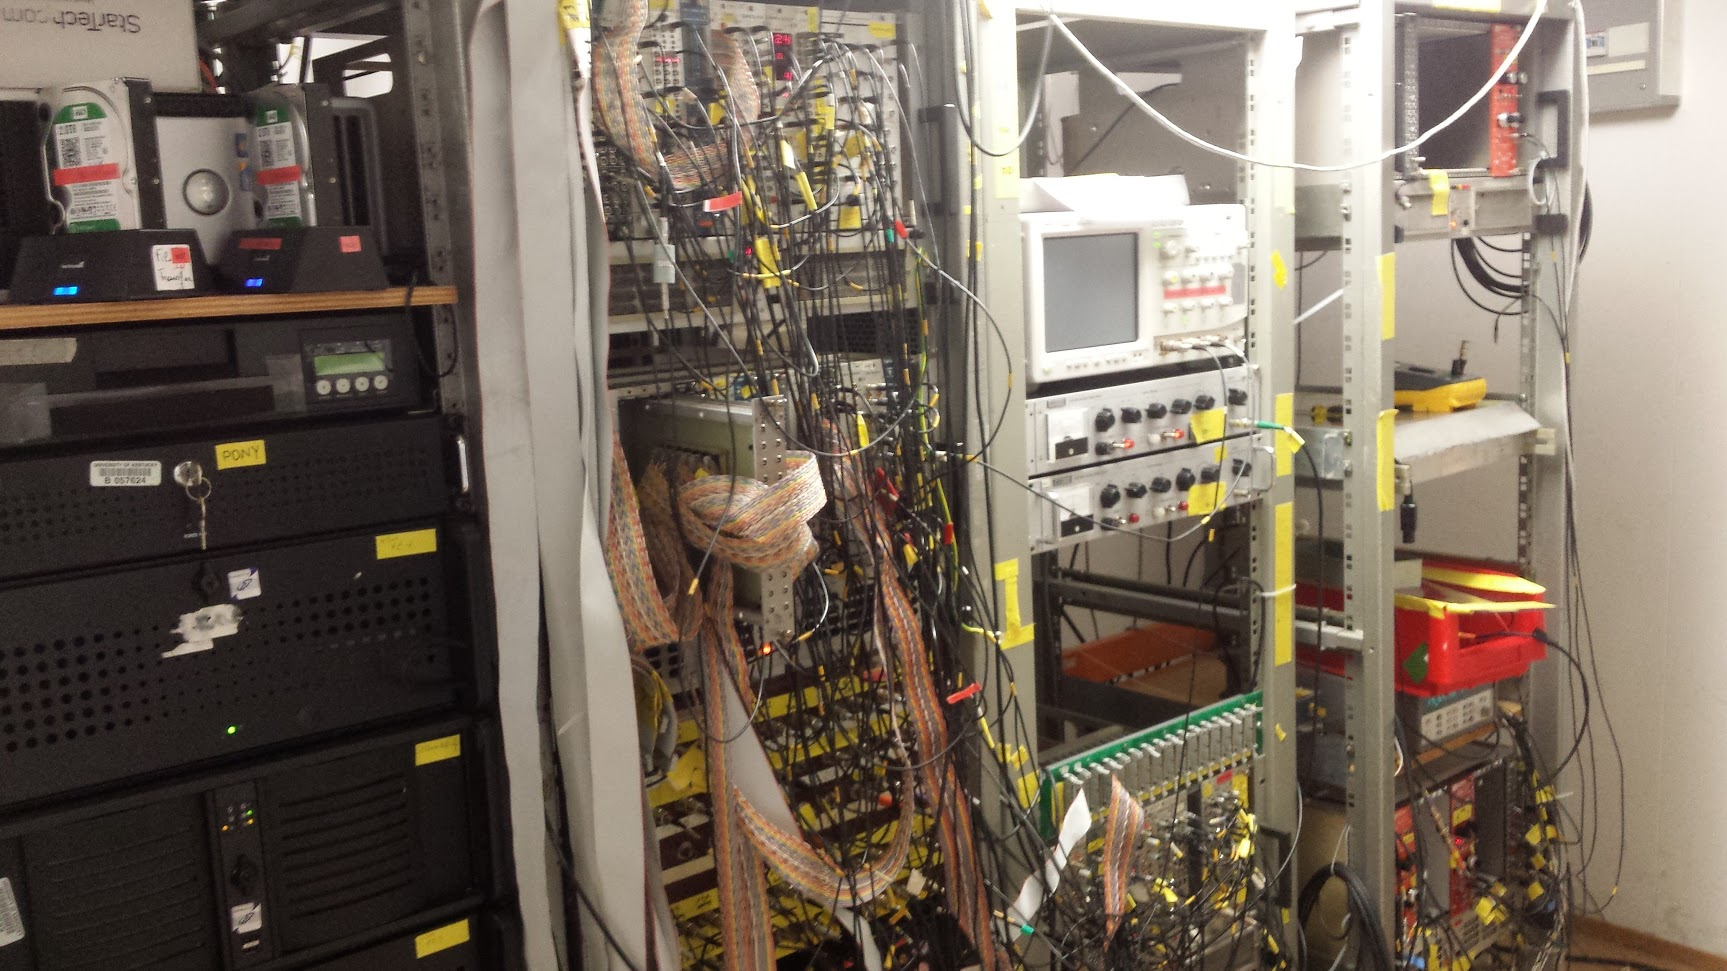
\includegraphics[height=0.6\textheight]{figures/daq.jpg} \\
  \end{itemize}
\end{frame}


\begin{frame}{Master Clock}{MuSun}
  \begin{itemize}
  \item {
  Scientific integrity: master clock blinding to avoid \say{human error} in estimating the Systematic Uncertainty (\textbf{accuracy}).
  }
  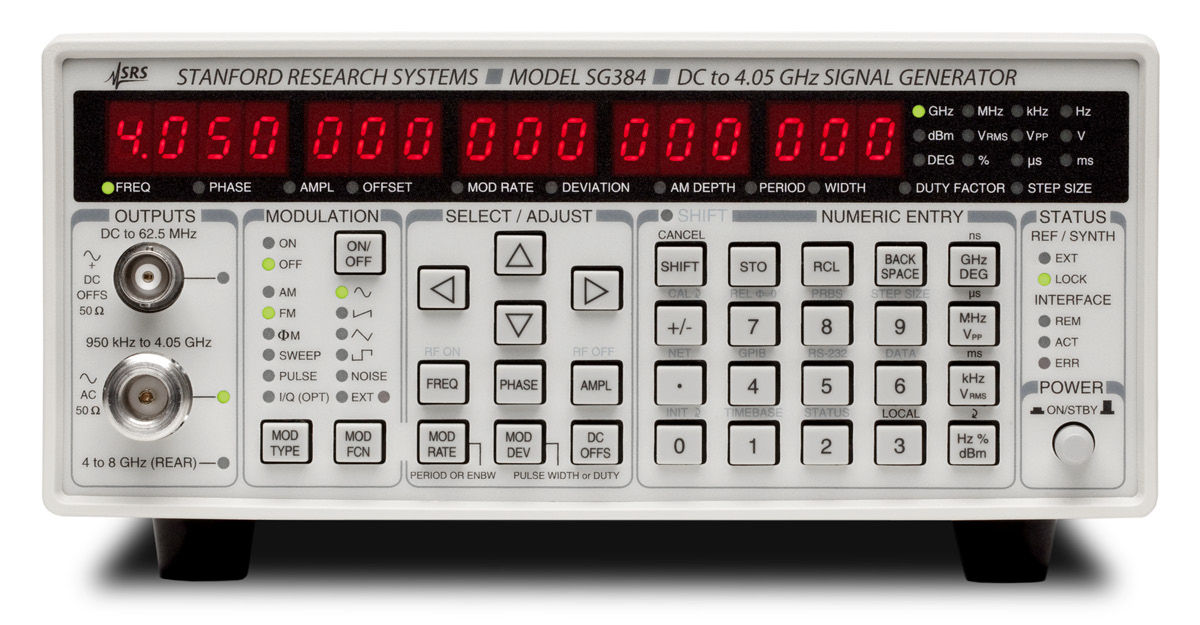
\includegraphics[height=0.4\textheight, width=0.9\textwidth]{figures/signal.jpg} \\
  \end{itemize}
  \let\thefootnote\relax\footnotetext{Image courtesy of the Stanford Research Systems.}
\end{frame}

\begin{frame}{Summer Student Involvement}{MuSun}
\begin{itemize}
\item Initial experiment set-up (3 weeks) 
\item Ensuring continuous data taking 
\item Calibration of 64 scintillation electron detectors 
\item Testing 8 neutron detectors
\item Beam tuning
\item Maintenance of beamline components

\item \textbf{Night shifts!}
\end{itemize}

    
\end{frame}


%%%%%%%%%%%%%%%%%%%%%%%%%%%%%%%%%%%%%%%%%%%%%%%%%%%%%%%%%%%%%%%%%%%%
\section{Overview of Fermilab g-2 (E989) experiment}
\subsection{Phenomenology of the Dipole Moments of the Muon}
\subsection{Proposed Experimental Methodology}

\begin{frame}{Overview}{g-2}
\begin{block}{Aim}
To measure the muon anomalous magnetic moment (AMM) to 140 parts per billion precision (ppb). 
\end{block}
The magnetic dipole moment (MDM) is given by
\begin{equation}
\boldsymbol{\mu}=g_{\mu}\left(\frac{q}{2m_{\mu}}\right) \boldsymbol{s},
\label{eq:mdm}
\end{equation}
where $g_{\mu}$ is the gyromagnetic ratio of the muon. While the AMM is given by
\begin{equation}
a_{\mu}=\frac{g_{\mu}-2}{2}.
\label{eq:AMM}
\end{equation}
The current \textbf{calculation} of $a_{\mu}$ is 0.00116591803(49), with 440 ppb precision. A 5$\sigma$ disagreement between the measured and the theoretical value is a sign of physics beyond the Standard Model (BSM): supersymmetry (SUSY), additional gauge bosons, or extra dimensions. 
\end{frame}

\begin{frame}{Overview}{g-2}
The AMM measurement through the precision frequency
\begin{equation}
\boldsymbol{\omega_a}=-a_{\mu}\frac{e}{m_{\mu}}\boldsymbol{B}.
\end{equation}
\centering
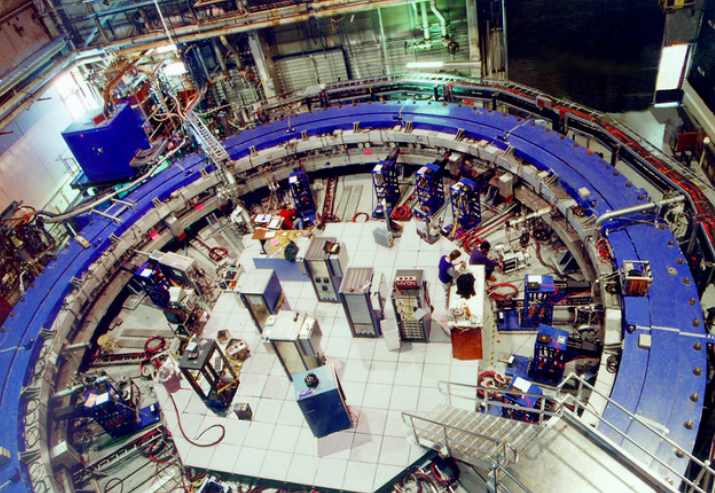
\includegraphics[height=.5\textheight]{figures/ring.png}
\let\thefootnote\relax\footnotetext{Image courtesy of the g-2 Collaboration [3].}
\end{frame}


\begin{frame}{Electric Dipole Moment}{g-2}
An electric dipole moment (EDM) measurement $> 2 \times 10^{-36}~e\cdot$cm would imply BSM physics through charge-parity (CP) violation, which can help explaining the matter-antimatter asymmetry in the Universe. \\
\centering
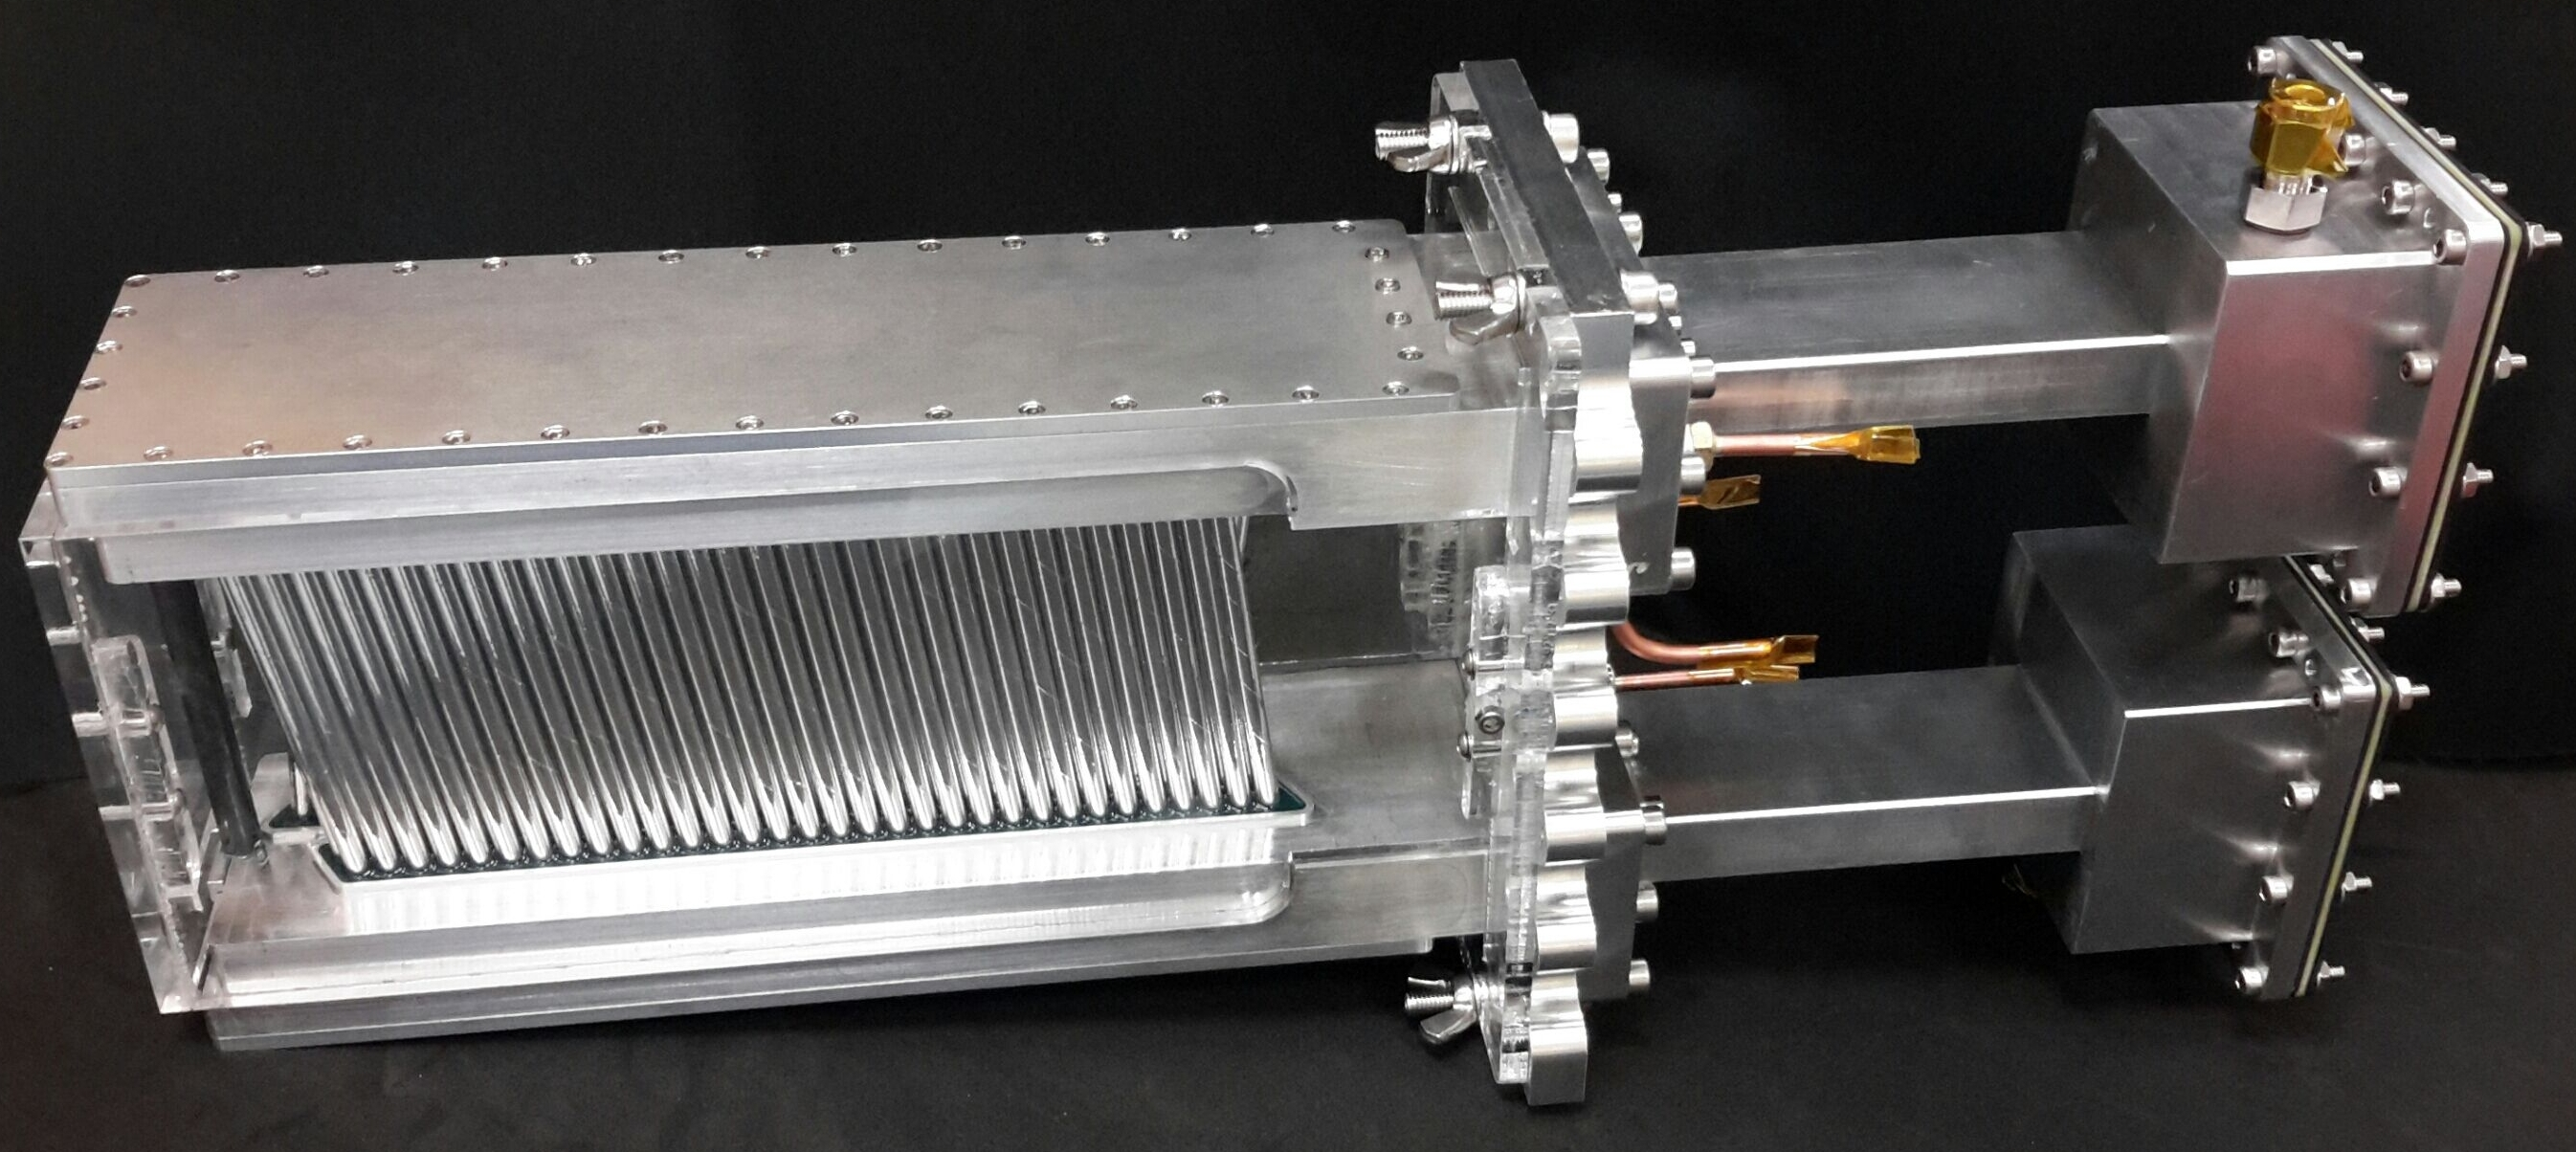
\includegraphics[height=.5\textheight]{figures/tracker.jpg}
\let\thefootnote\relax\footnotetext{Image courtesy of the g-2 Collaboration [3].}
\end{frame}
    

\begin{frame}{Master's Student Duties}{g-2}
\begin{itemize}
\item Data Analysis (testbeam) 
\item Hardware work:
\end{itemize}
\centering
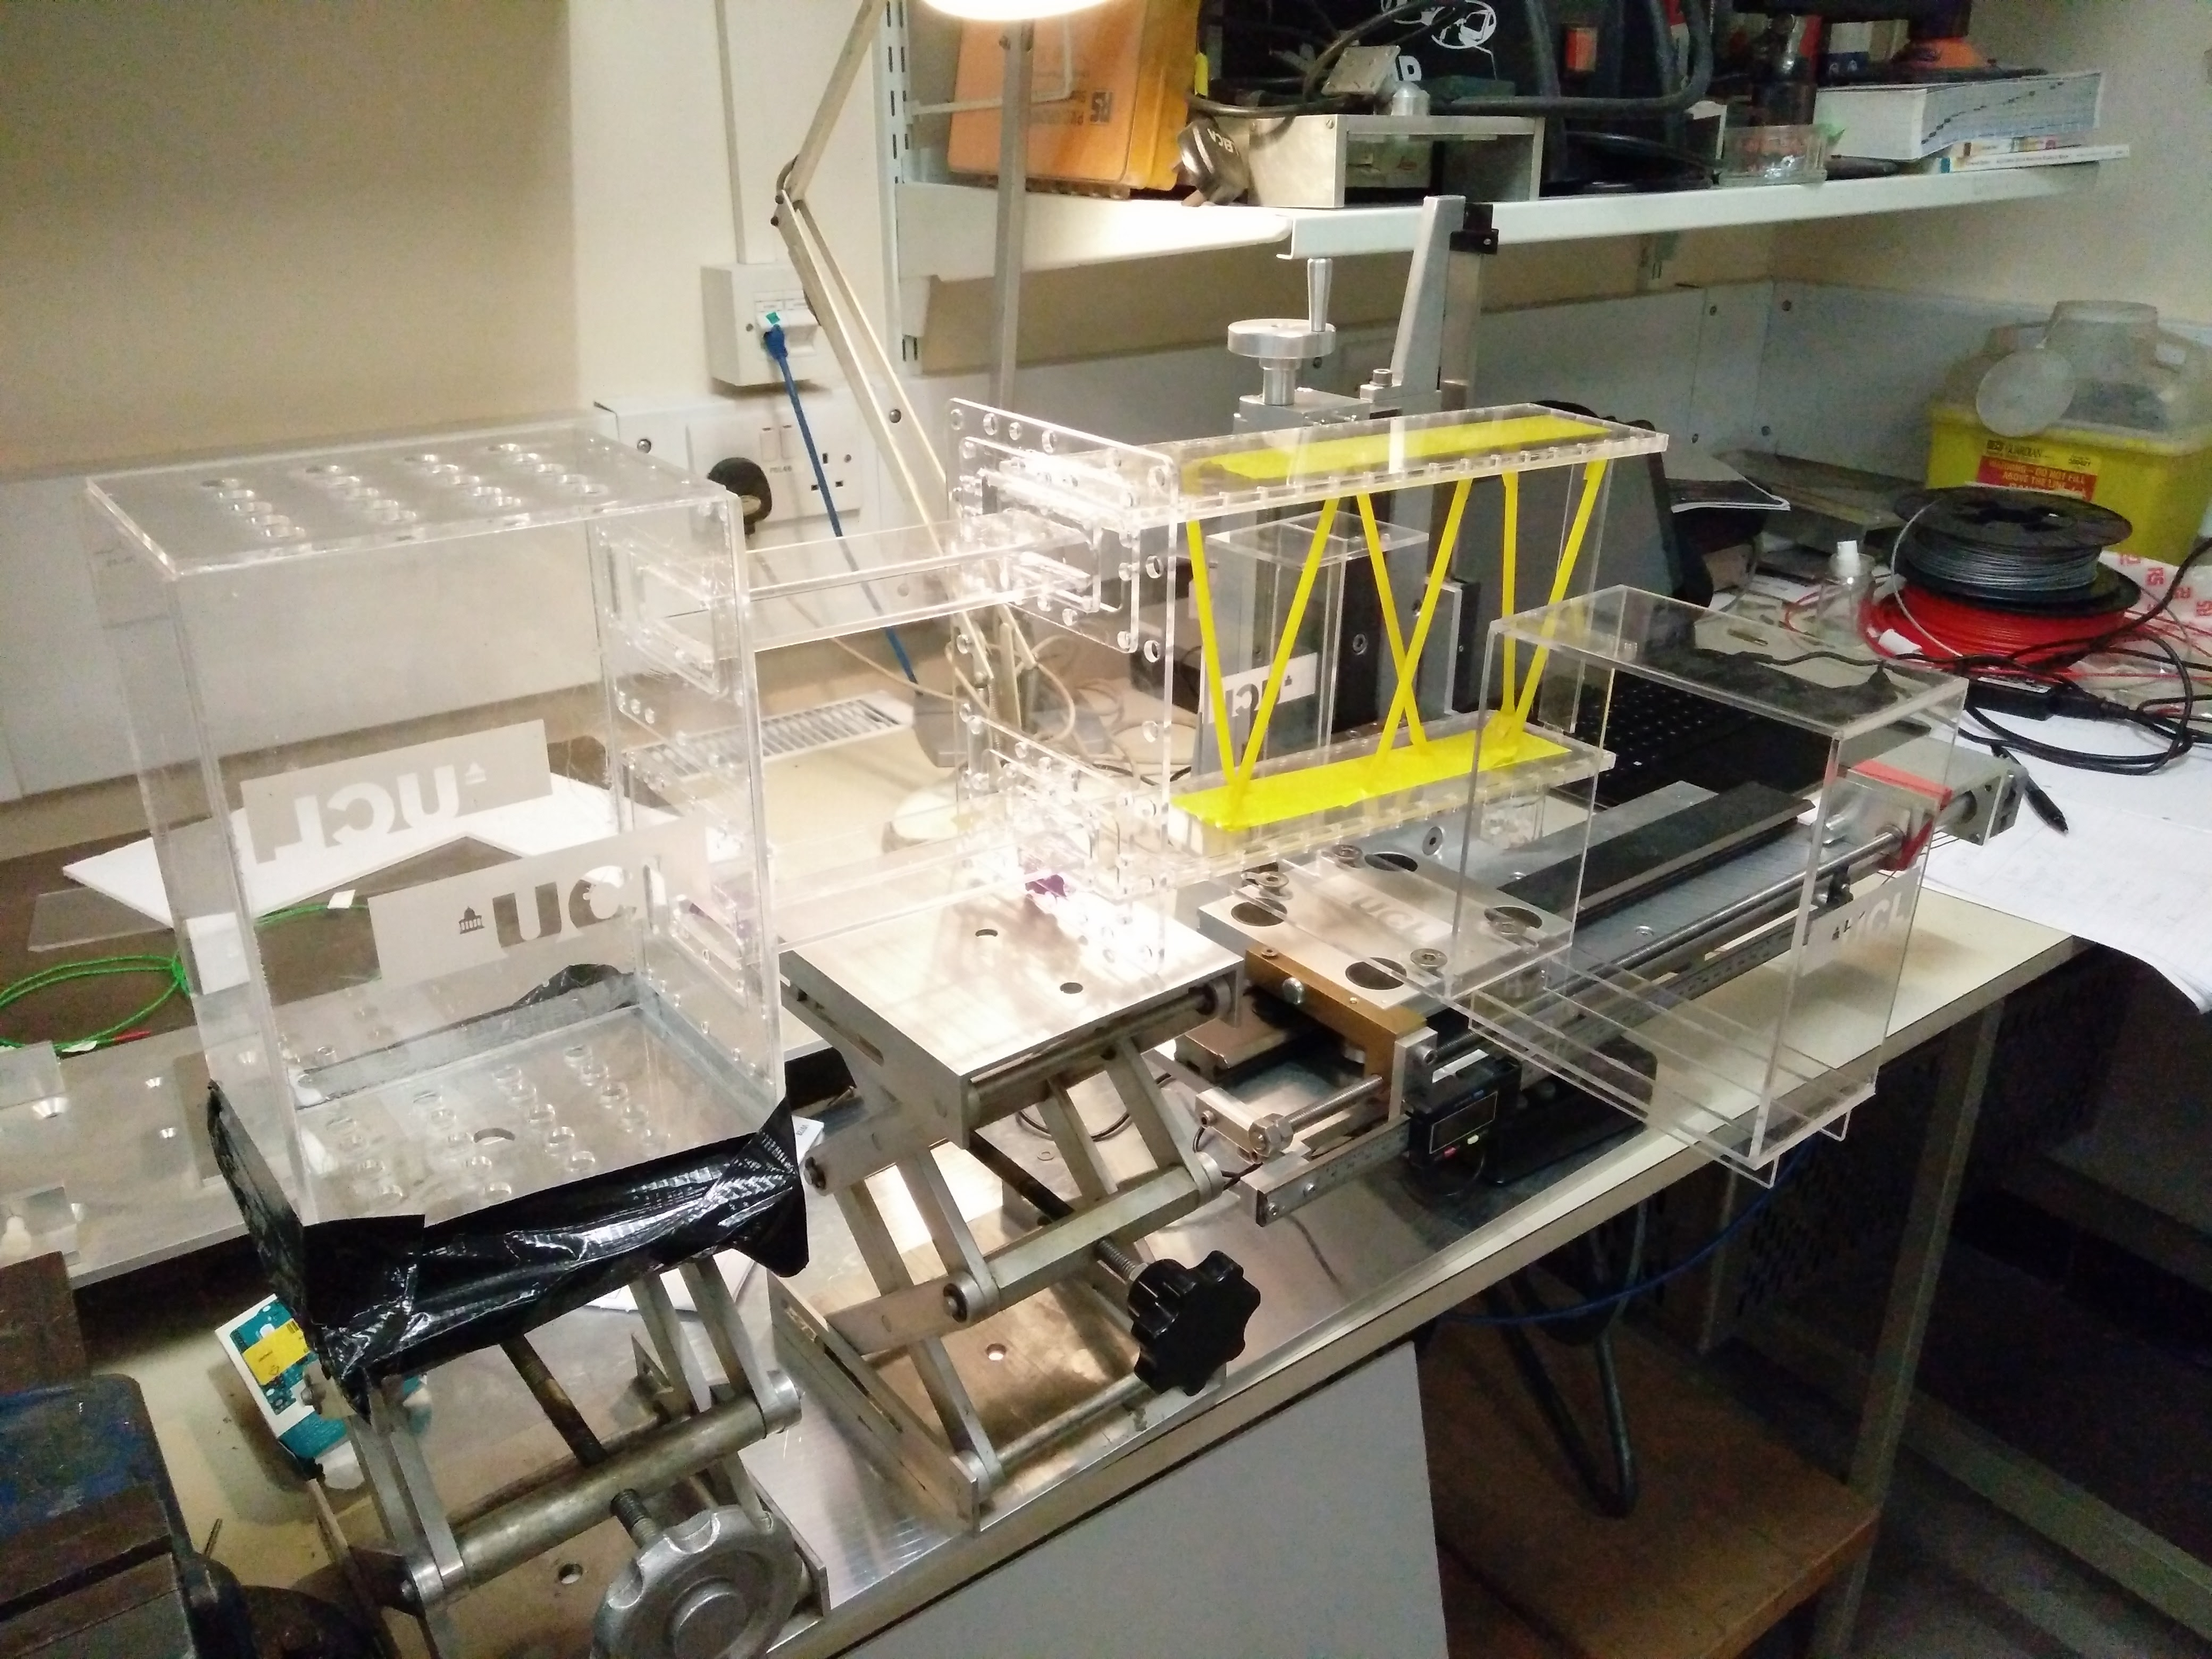
\includegraphics[height=.5\textwidth]{figures/stand.jpg}

\end{frame}

\begin{frame}{References:}{For Further Reading}
  \begin{thebibliography}{10}
    
  \beamertemplatearticlebibitems
  % Followed by interesting articles. Keep the list short. 

\bibitem{PMP}
     \newblock [1] {\em  Precision Muon Physics} \\
     T. Gorringe, D. Hertzog \\
    \href{http://arxiv.org/abs/1506.01465}{Available from the arXiv:1506.01465}

 \bibitem{MuSun}
     \newblock [2] {\em  Muon Capture on the Deuteron.} \\
     V. Andreev, et al. (MuSun Collaboration) \\
    \href{http://arxiv.org/pdf/1004.1754.pdf}{Available from the arXiv:1004.1754}
    
\bibitem{g-2}
     \newblock [3] {\em  Muon (g-2) Technical Design Report} \\
     J. Grange, et al. (E989 Collaboration) \\
    \href{http://arxiv.org/abs/1501.06858}{Available from the arXiv:1501.06858}
    



  \beamertemplatebookbibitems
  % Start with overview books.

%  \bibitem{Jon_Butterworth}
%   \newblock  [3] {\em Smashing Physics}. \\
%        Jon Butterworth \\
   %\href{http://www.theguardian.com/books/2014/may/02/smashing-physics-jon-butterworth-review-cern-higgs-boson-particle}{Review here}\\
%    \href{http://www.amazon.co.uk/Smashing-Physics-Jon-Butterworth/dp/1472210301}{Amazon link here}\\
 %   \href{http://www.richannel.org/smashing-physics}{See also the Royal Institution video lecture for free here}

      \end{thebibliography}
\end{frame}



\section*{Backup Slides}

\begin{frame}{Backup Slides}
    
\end{frame}

\begin{frame}{Summer Research Work at PSI}
\begin{block}{How to Apply:}
Summer Research Student or Trainee position.\\
Find a research area and group/experiment of interest:\\
\url{https://www.psi.ch/science/research-departments-and-labs}
Contact the relevant member of staff, and \\
1) Explain why are you excited in this area? \\
2) How it can benefit your future plans? \\
3) Attach CV \\
4) Attach any relevant academic work (e.g. Literature Review)
\end{block}

\end{frame}



\begin{frame}{Travelling in Switzerland}
\centering
\begin{columns}[onlytextwidth]
\centering
  \begin{column}{0.5\textwidth}
  \centering
  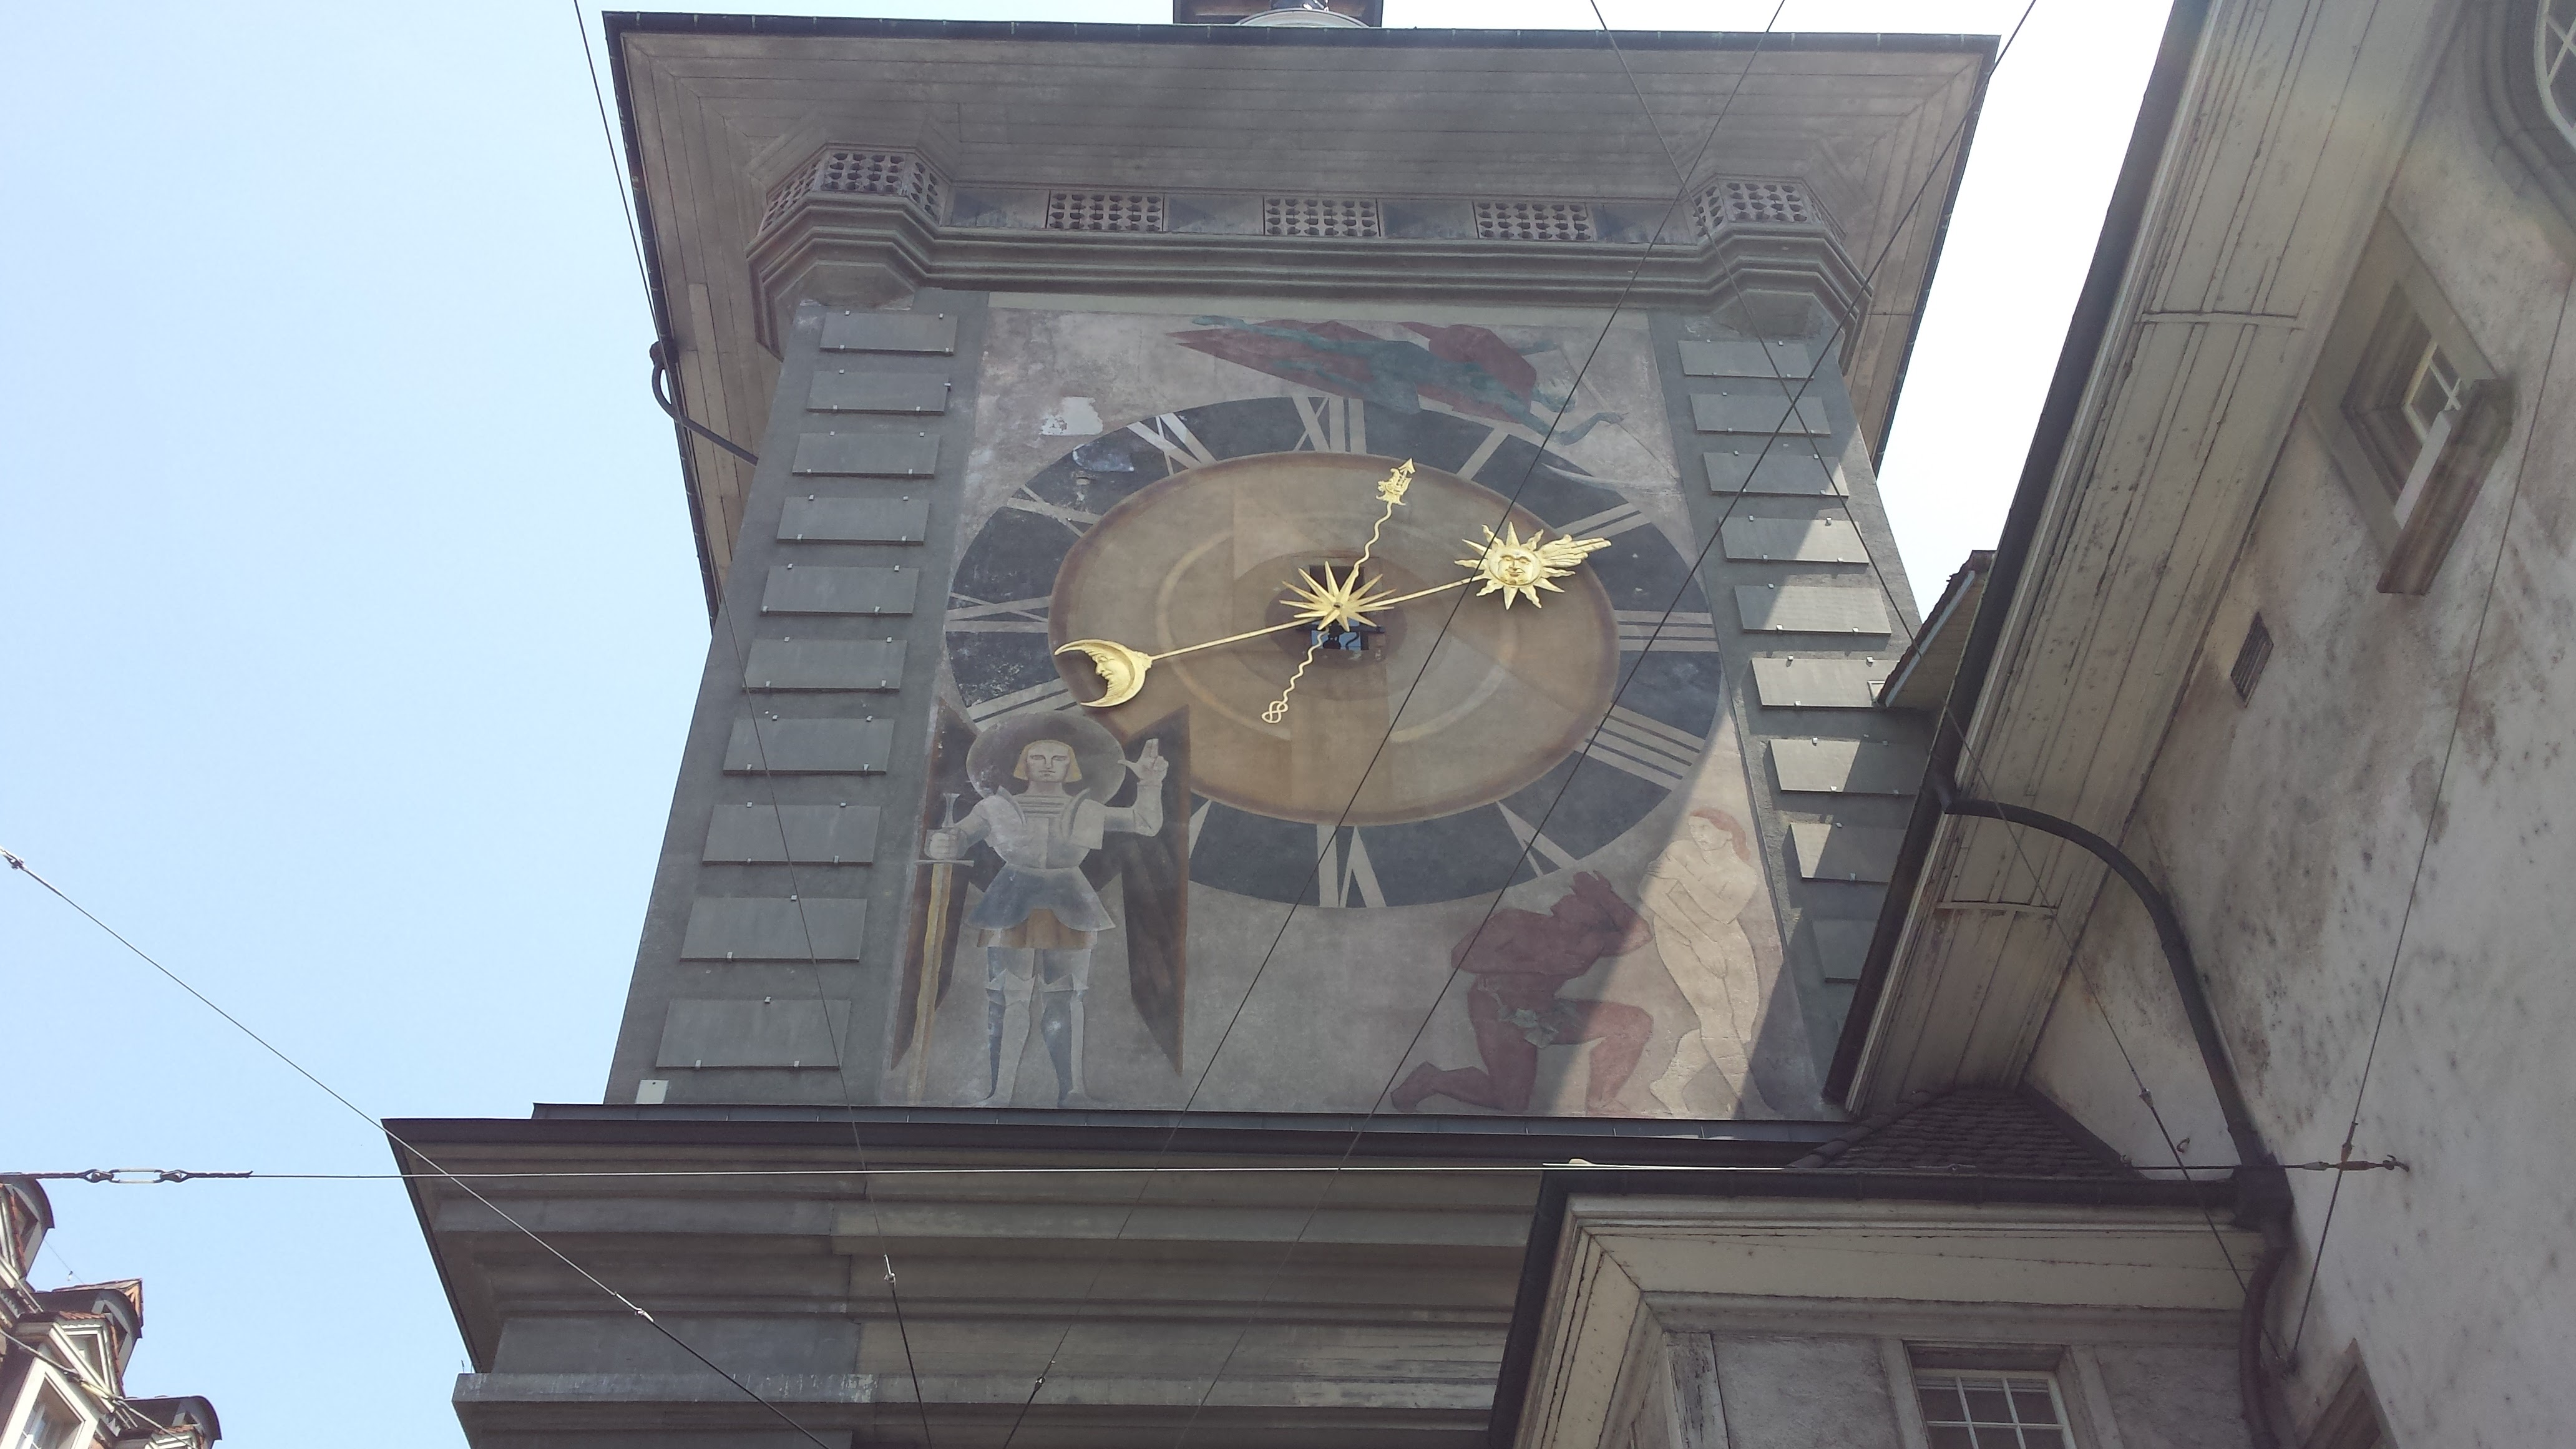
\includegraphics[height=0.4\textheight, width=0.85\textwidth]{figures/pr1.jpg} \\
  \centering
 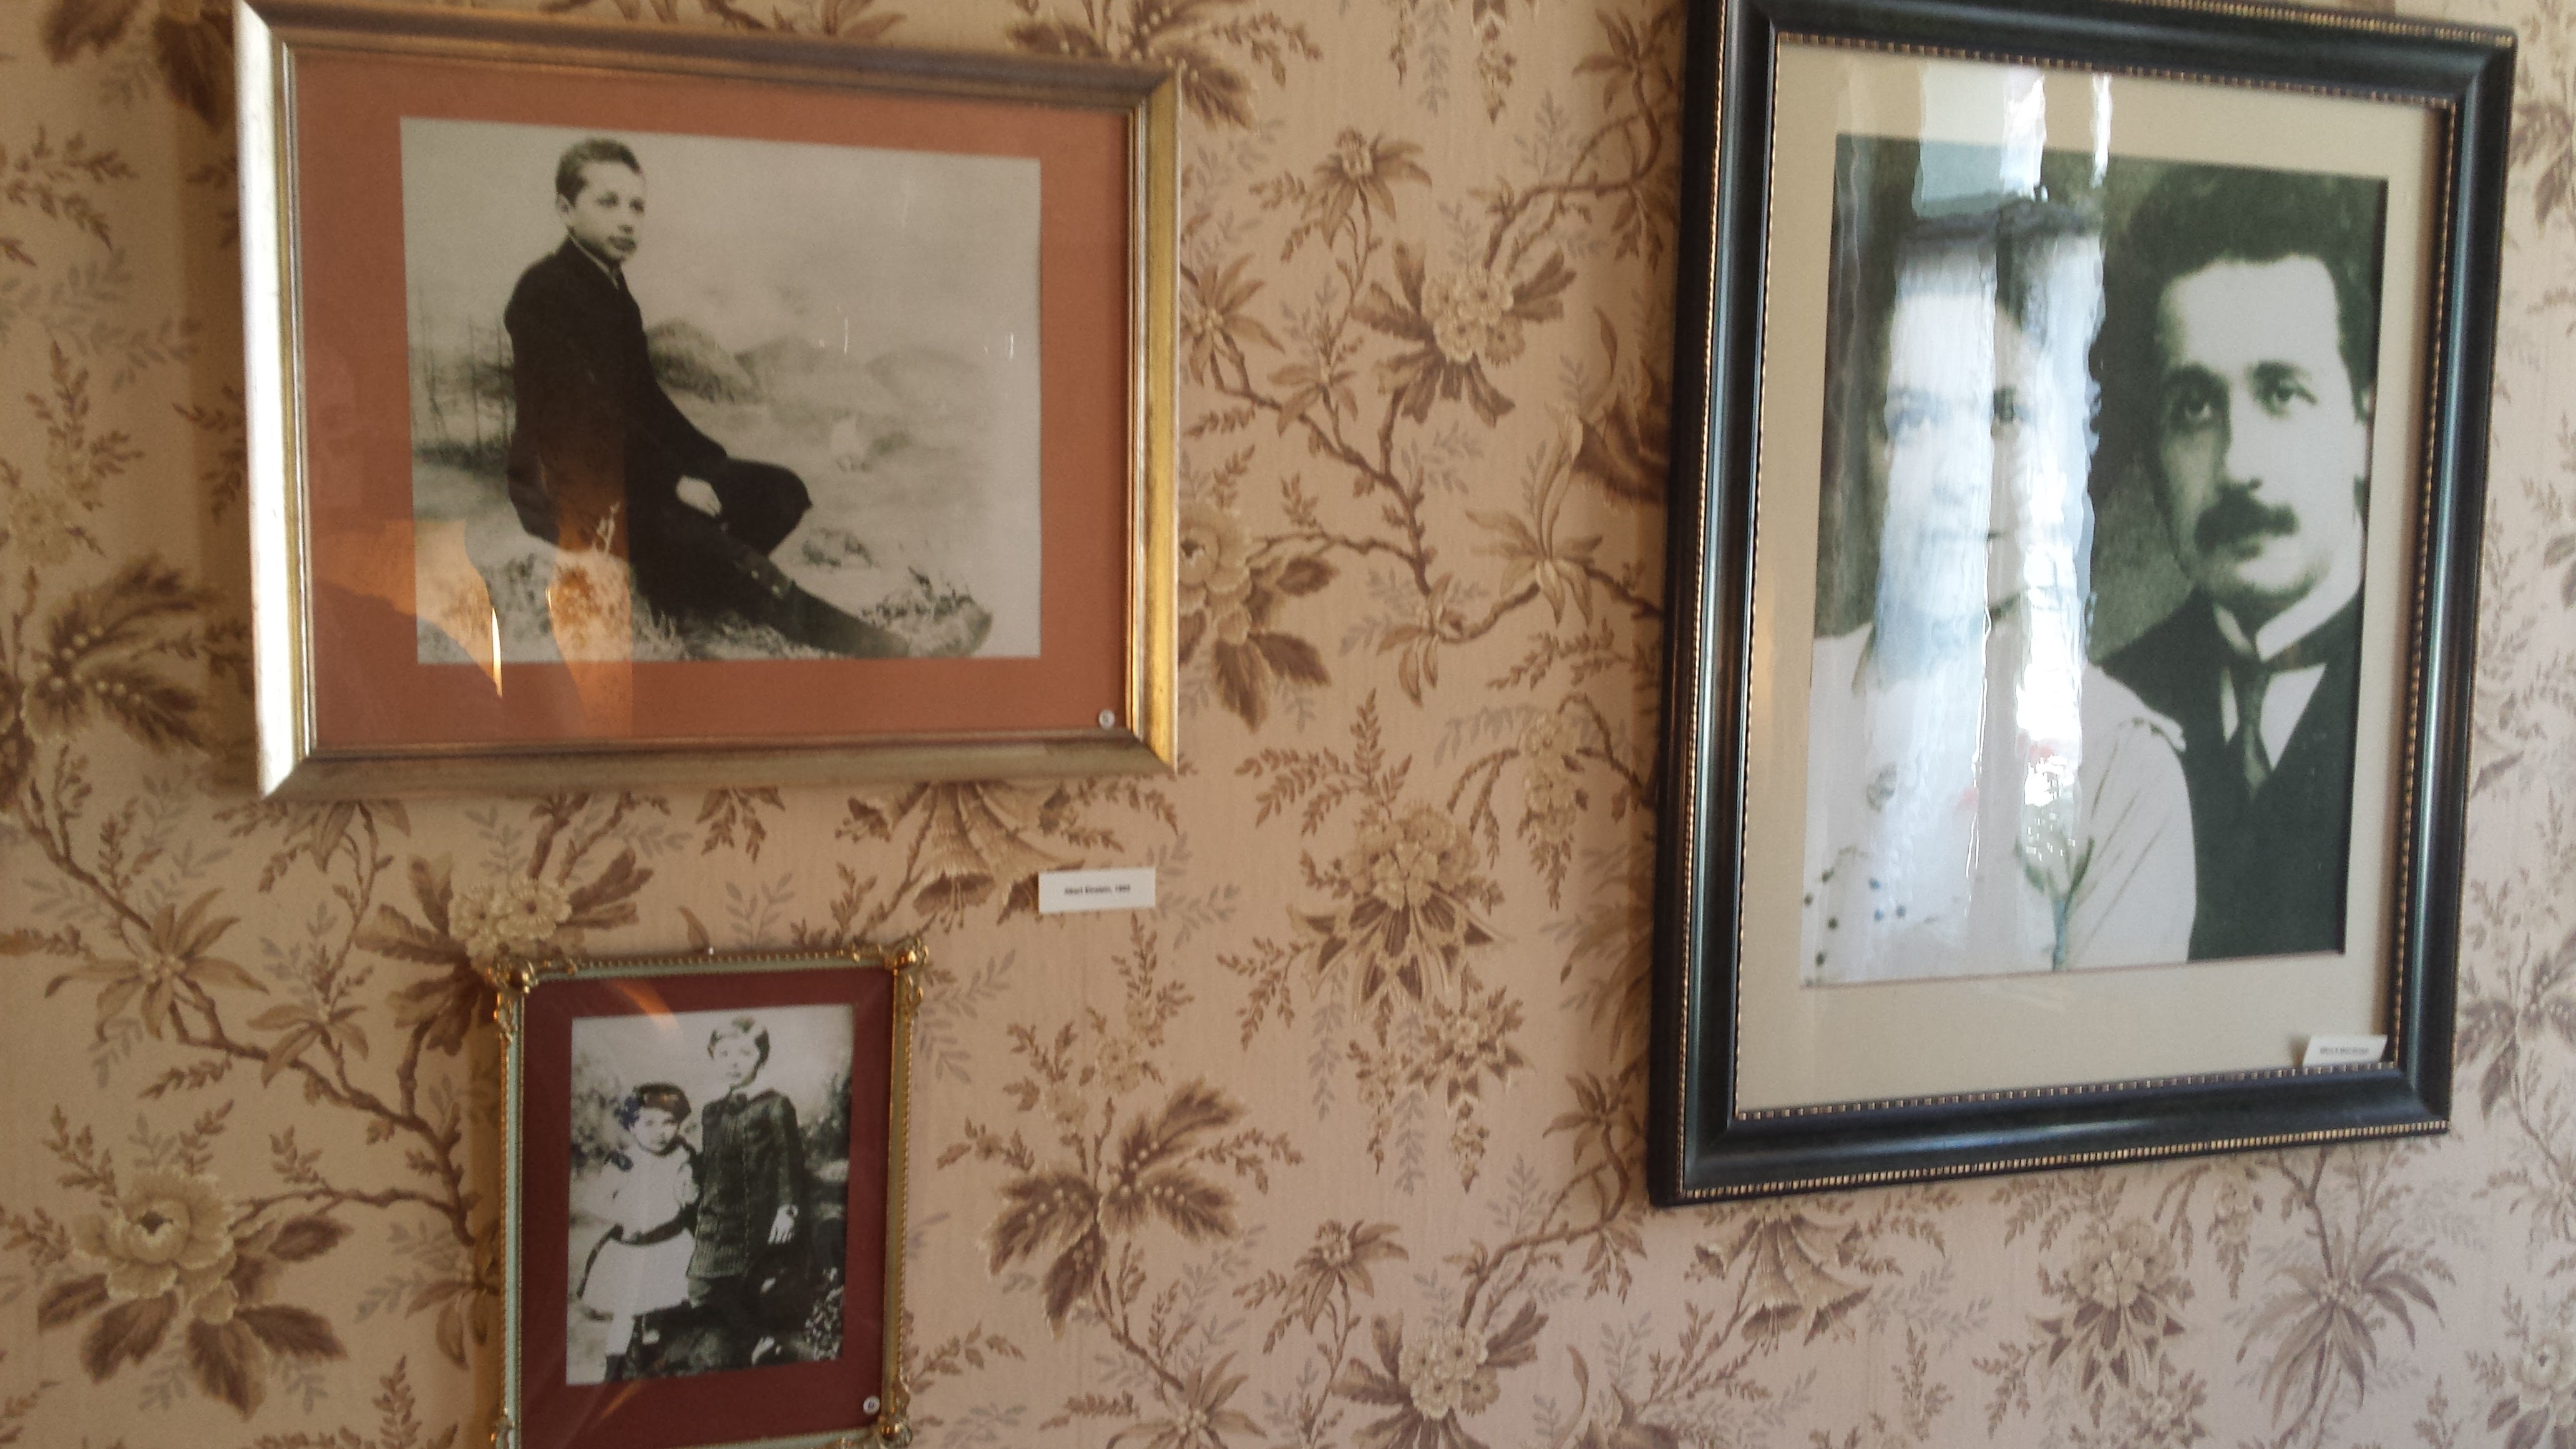
\includegraphics[height=0.4\textheight, width=0.85\textwidth]{figures/pr2.jpg}\\
  \end{column}
  \centering
  \begin{column}{0.5\textwidth}
  \centering
  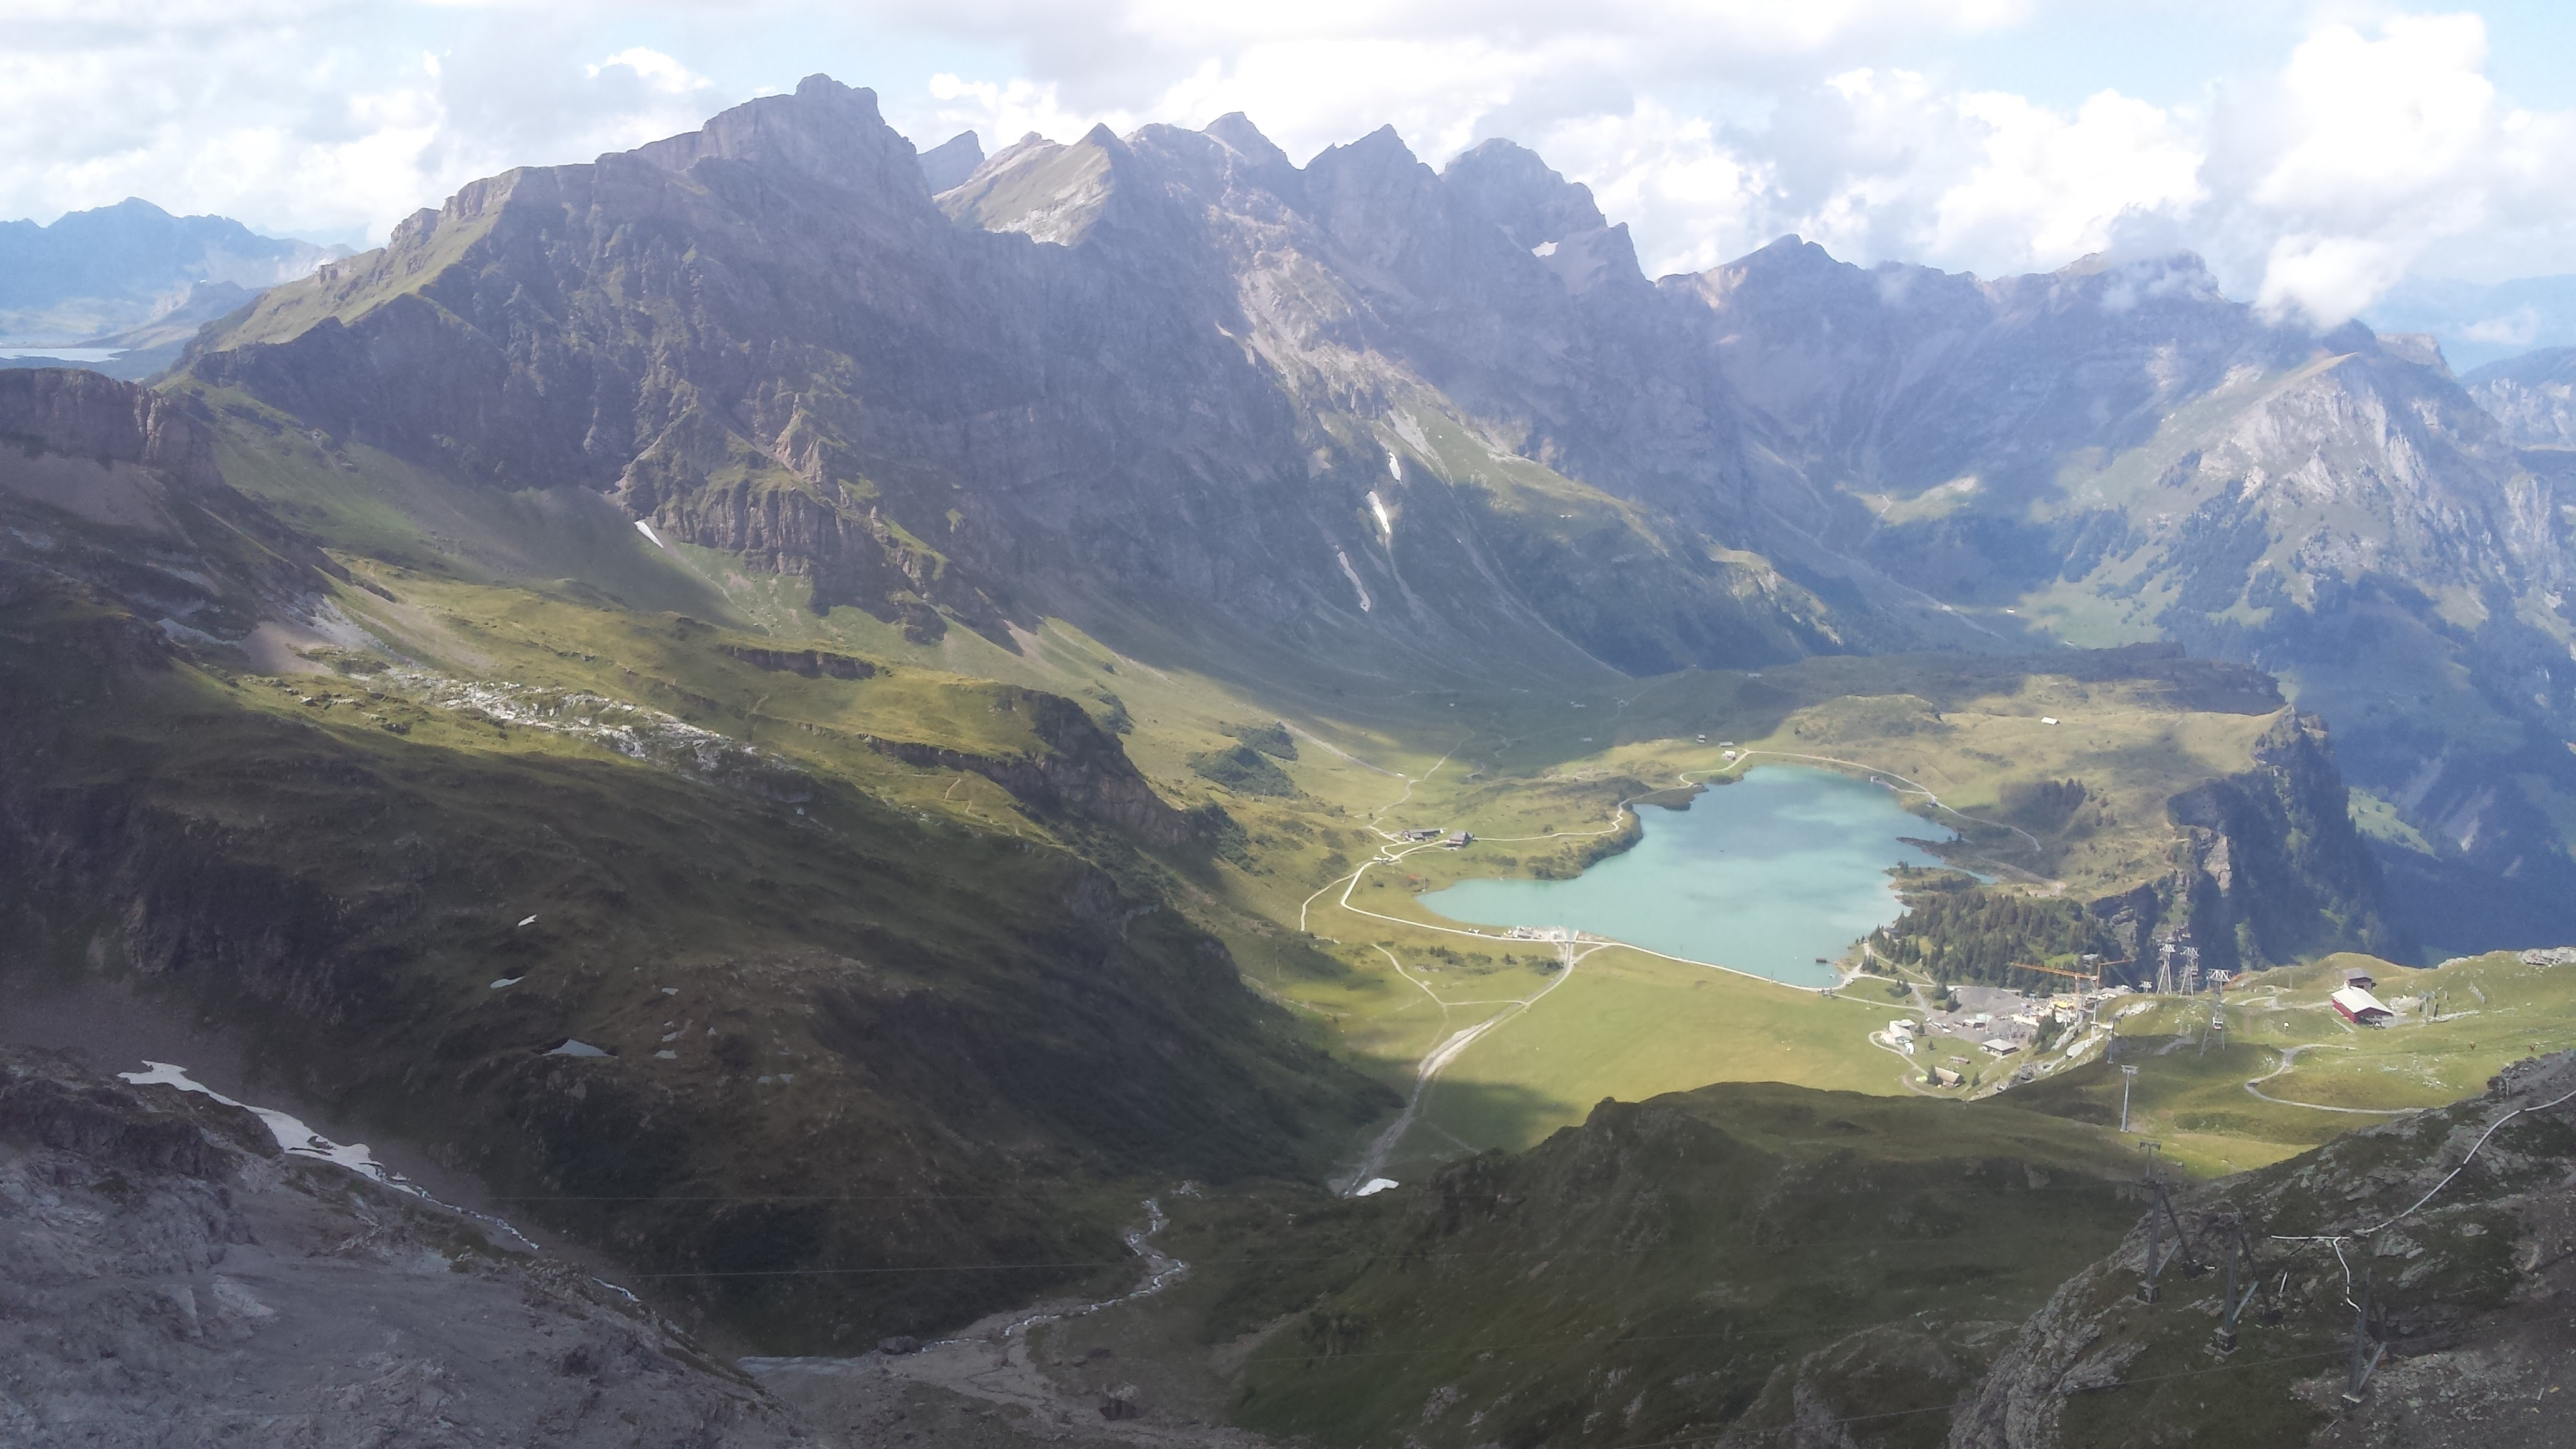
\includegraphics[height=0.4\textheight, width=0.85\textwidth]{figures/pr3.jpg} \\
  \centering
  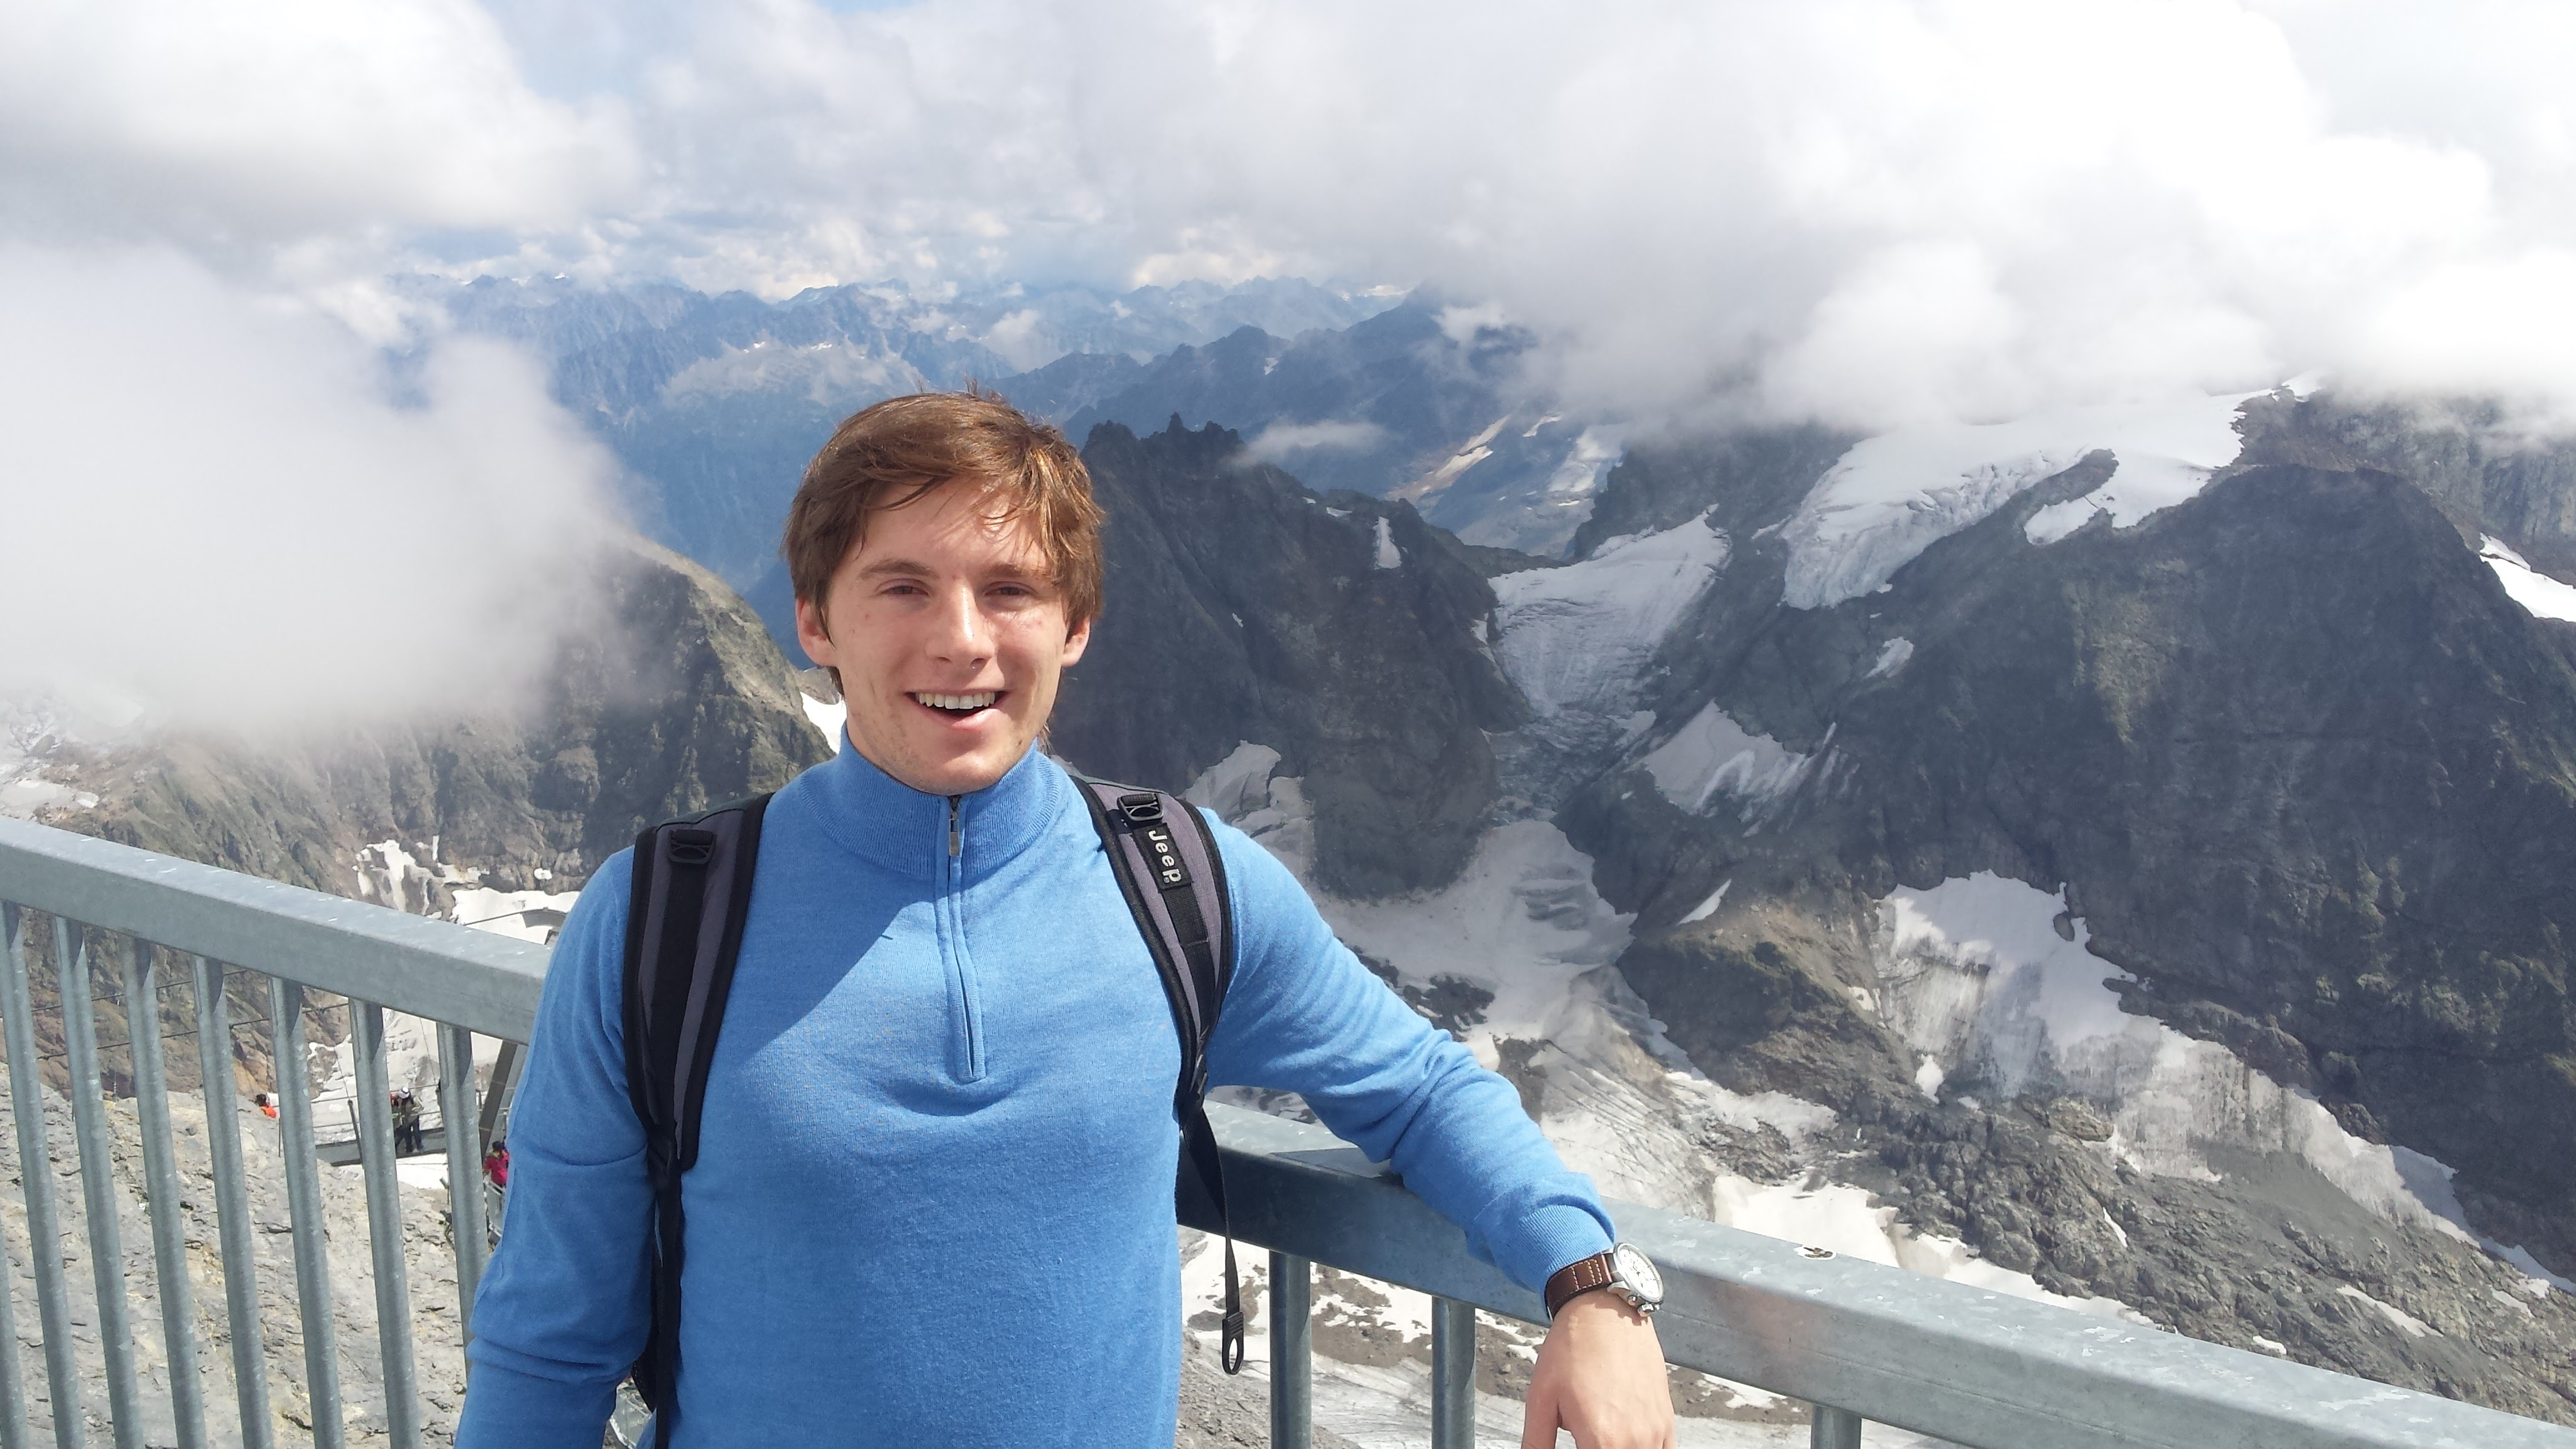
\includegraphics[height=0.4\textheight, width=0.85\textwidth]{figures/pr4.jpg}
  \end{column}
  \end{columns}
 
\end{frame}



% Placing a * after \section means it will not show in the
% outline or table of contents.


% All of the following is optional and typically not needed. 
%\appendix
%\section<presentation>*{\appendixname}
%\subsection<presentation>*{For Further Reading}

%\begin{frame}[allowframebreaks]
 % \frametitle<presentation>{For Further Reading}



\end{document}


